\documentclass[traditabstract]{aa}

\usepackage[stable]{footmisc}
\usepackage{graphicx}
\usepackage[varg]{txfonts}
\usepackage{hyperref}
\usepackage{natbib,twoopt}
\usepackage{lscape}
\usepackage{hyperref} 
\usepackage{subcaption}
\usepackage{nicefrac}
\bibpunct{(}{)}{;}{a}{}{,} 

\makeatother\bibpunct[, ]{(}{)}{;}{a}{}{,}

\bibliographystyle{./bibtex/aa}

\newcommand{\farc}{\hbox{$.\!\!^{\prime\prime}$}} 
\newcommand{\ergA}{$\rm{erg\,c m^{-2}\,s^{-1}\,\AA\,^{-1}}$} 
\newcommand{\erg}{$\rm{erg\,cm^{-2}\,s^{-1}}$} 
\newcommand{\kms}{$\rm{km\,s^{-1}}$}
\newcommand{\hb}{H$\beta$} 
\newcommand{\ha}{H$\alpha$}
\newcommand{\hg}{H$\gamma$} 
\newcommand{\hd}{H$\delta$} 
\newcommand{\hi}{\mbox{H\,{\sc i}}} 
\newcommand{\hii}{\mbox{H\,{\sc ii}}} 
\newcommand{\ebv}{$E_{B-V}\,$} 
\newcommand{\oh}{$12+\log(\mathrm{O/H})$}

\newcommand{\hei}{\ion{He}{i}} 
\newcommand{\oi}{[\ion{O}{i}]} 
\newcommand{\sii}{[\ion{S}{ii}]} 
\newcommand{\siii}{[\ion{S}{iii}]} 
\newcommand{\oii}{[\ion{O}{ii}]}
\newcommand{\cii}{[\ion{C}{ii}]} 
\newcommand{\oiii}{[\ion{O}{iii}]}
\newcommand{\neiii}{[\ion{Ne}{iii}]}
\newcommand{\nii}{[\ion{N}{ii}]} 
\newcommand{\griz}{$g' r' i' z'$}
\newcommand{\JHK}{$JHK_{\rm{s}}$}
\newcommand{\gK}{$g' r' i' z' JHK_{\rm{s}}$}
\newcommand{\Msun}{$M_\odot$}
\newcommand{\Msunyr}{$M_\odot\,\rm{yr}^{-1}$}
\newcommand\nodata{ ~$\cdots$~ }

\begin{document}
\title{Hot gas around SN~1998bw - the progenitor from its environment\thanks{Based on observations at ESO, Program ID: 095.D-0172}}
\titlerunning{Hot gas around SN98bw}

\author{T.~Kr\"{u}hler\inst{1}
\and H.~Kuncarayakti\inst{2, 3}
\and P.~Schady \inst{1} 
\and J.~Anderson \inst{4}
\and L.~Galbany \inst{5}
\and J.~Gensior \inst{6}}

\institute{Max-Planck-Institut f\"{u}r extraterrestrische Physik, Giessenbachstra\ss e, 85748 Garching, Germany
\and Millennium Institute of Astrophysics, Casilla 36-D, Santiago, Chile
\and European Southern Observatory, Alonso de C\'{o}rdova 3107, Vitacura, Casilla 19001, Santiago 19, Chile 
\and Departamento de Astronom\'ia, Universidad de Chile, Casilla 36-D, Santiago, Chile
\and Pittsburgh Particle Physics, Astrophysics, and Cosmology Center, Physics and Astronomy Department, University of Pittsburgh, Pittsburgh, PA 15260, USA.
}

\abstract{Spatially-resolved spectroscopy of the environment of explosive transients carries detailed information about the physical properties of the stellar population that gave rise to the explosion, and thus the progenitor star itself. Here, we use  observations from the novel integral-field spectrograph MUSE of the galaxy hosting GRB~980425 (SN~1998bw) to constrain the stellar age and oxygen abundance at the explosion site. The immediate environment ($\sim$~100~pc) of GRB~980425 is consistent with a progenitor of zero-age main-sequence mass between 25\,M$_{\odot}$ and 40\,M$_{\odot}$ and metallicity \oh$\sim$8.1 (0.25\,$Z_\odot$). This oxygen abundance is somewhat lower than the one of a nearby, extremely young, \hii-region (\oh$\sim$8.3) and an integrated measurement over the whole galaxy (\oh$\sim$8.3). We demonstrate that simple empirical strong-line methods based on \oiii\,and/or \nii\, are inadequate to produce accurate maps of oxygen abundance at the level of detail of our MUSE observation and show that these methods over-/underestimate \oh\,at low/high ionization parameter. The metallicity gradient in ESO184-G82 is -0.06\,dex\,kpc$^{-1}$, indicating that the typical offsets of at most few kpc for cosmological GRBs have a small impact for high-redshift measurements on average. Similarly, the GRB/SN site spectrum returns broadly comparable physical parameters than what would be inferred through an unresolved spectrum, which is typically obtained for high-redshift galaxies.}

\keywords{Gamma-ray burst: general, individual: GRB~980425, Galaxies: ISM, star formation, abundances}
\maketitle

\section{Introduction}
\label{sec:Intro}

Line emission from recombination of ionized hydrogen, or decay of collisionally-excited states of metal ions plays a fundamental role in modern astrophysics. The absolute and relative intensities of these transitions crucially depend on the ionizing source, the electron density in the plasma, the ionization state of the elements, and gas-phase abundances \citep{1989agna.book.....O}. This makes emission-line spectra of astronomical sources one of the most elementary diagnostics of galaxy formation and evolution \citep[e.g.][]{2004ApJ...613..898T, 2006ApJ...644..813E, 2009ApJ...706.1364F}. The total intensity of the hydrogen recombination lines, for example, is proportional the number of O-type stars, and thus traces the star-formation rate at timescales of $\sim 10$\,Myrs \citep[e.g.][]{1998ARA&A..36..189K}. The continuum emission at the wavelength of \ha\, in turn originates from B- or A-type stars, which makes the \ha\, equivalent width (EW) a good tracer of the age of the stellar population.

Metal abundances have been measured through ratios of prominent emission lines from ions such as O$^{+}$, O$^{2+}$, N$^{+}$, S$^{+}$ and/or recombination lines of hydrogen \citep{1979MNRAS.189...95P, 1979A&A....78..200A}. Given their fundamental importance in galaxy evolution and cosmology, these abundance determinations through nebular emission lines have been the focus of a large body of literature \citep[e.g.][]{2004ApJ...617..240K, 2005ApJ...631..231P, 2006A&A...454L.127S, 2006A&A...448..955I, 2008ApJ...681.1183K}.

It is thus immediately clear that an emission-line spectrum of cosmological sources carries detailed information about the underlying stellar population and thus has been used to infer properties not only of galaxies but also of the progenitors of explosive transients \citep[see e.g.][for a review]{2009ARA&A..47...63S}. Global \citep[e.g.][]{2008ApJ...673..999P, 2011MNRAS.412.1441L} or local \citep[e.g.][]{2010MNRAS.407.2660A, 2011ApJ...731L...4M, 2011A&A...530A..95L} properties of nearby supernovae hosts, as well as cosmological $\gamma$-ray bursts \citep[e.g.][]{2007A&A...464..529W, 2012A&A...546A...8K, 2013ApJ...774..119G} or super-luminous supernovae \citep[e.g.][]{2013ApJ...763L..28C, 2014ApJ...787..138L, 2014arXiv1409.8331L, 2016arXiv160408207P} have likewise been used to compare progenitor models with the expected environments. 

A fundamental assumption of all these studies is the hypothesis that there is a tight relation between the primary measurements of gas-phase oxygen abundance or age of \hii\,regions and metallicity or life time and thus initial mass of the progenitor star. Clearly, this link is most robust when coming from an analysis of the co-spatial stellar population. Integral-field spectroscopy (IFS) with high angular resolution is thus arguably the most comprehensive way of studying the environments of explosive transients. Low-redshift galaxies hosting supernovae (SN), for example, are hence ideal targets for state-of-the-art integral-field units \citep[IFUs, e.g.][]{2013AJ....146...30K, 2014A&A...572A..38G}.

In contrast to nearby SNe, the vast cosmological distances of GRBs \citep[e.g.][]{2009ApJS..185..526F, 2009Natur.461.1254T, 2015A&A...581A.125K} have always posed serious limitations on using IFS for GRB-selected galaxies. Only few GRBs are close enough such that the spatial resolution with modern ground-based instrumentation yields constraints on scales better than a kpc. Seminal work on spatially-resolved spectroscopy for nearby GRB hosts could be obtained for only a handful cases using long-slit spectroscopy \citep[e.g.][]{2008ApJ...676.1151T, 2011ApJ...739...23L, 2015A&A...579A.126S} or the previous generation of IFUs \citep{2008A&A...490...45C, 2014MNRAS.441.2034T}. 

\begin{figure}
\begin{subfigure}{.47\textwidth}
  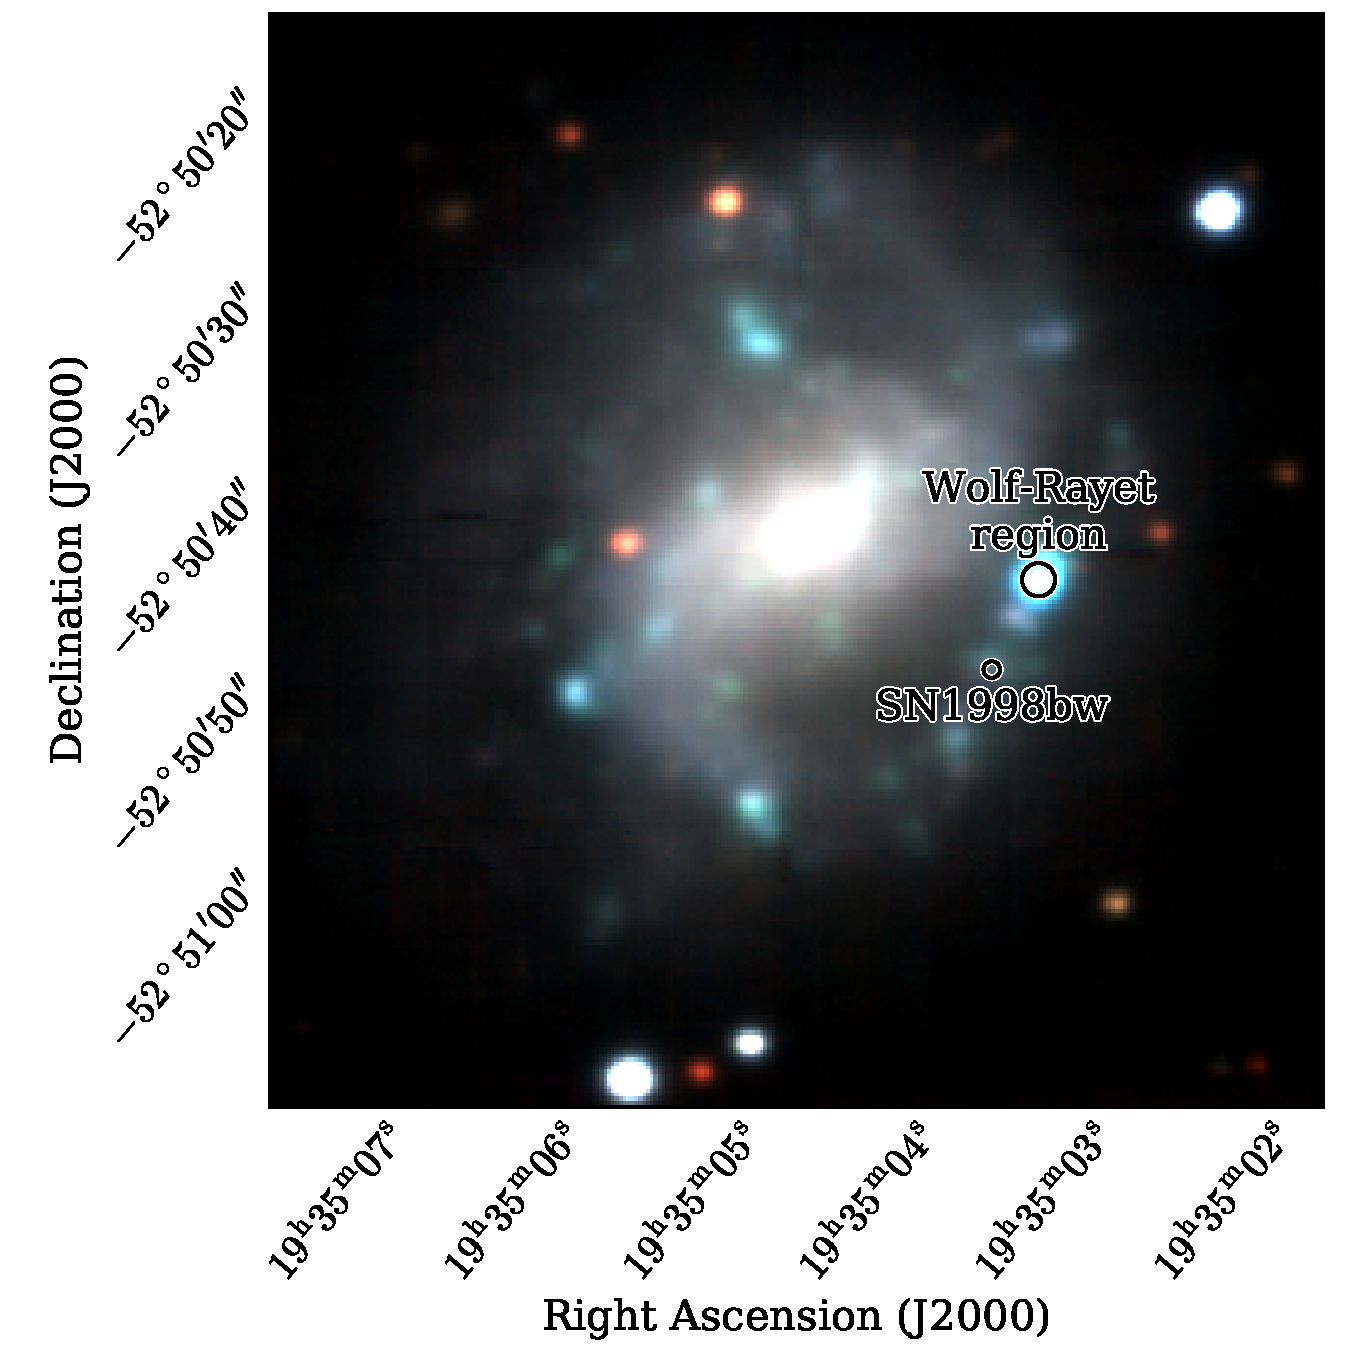
\includegraphics[width=0.999\linewidth]{Figs/MUSE_SN1998bw_RGB.pdf}
\end{subfigure}
\caption{Reconstructed image from the MUSE data cube. False-color composite from reconstructed $VRI$-band images. The image spans approximately 55" by 55", or 10 by 10 kpc. One MUSE spaxel corresponds to 35~pc. The effective spatial resolution is given by the point spread function with a FWHM of approximately 0\farc{9}.}
\label{fig:Host}
\end{figure}

The focus of this article are our new observations of the poster-child of the GRB/SN connection, GRB\,980425/SN\,1998bw obtained with the Multi-Unit Spectroscopic Explorer (MUSE, \citealp{2010SPIE.7735E..08B}). GRB\,980425 is the closest GRB yet discovered and both the GRB \citep[e.g.][]{1998Natur.395..670G, 1998Natur.395..663K}, the SN \citep[e.g.][]{1998Natur.395..672I, 2001ApJ...555..900P, 2006ApJ...640..854M} and host galaxy \citep[e.g.][]{2000ApJ...542L..89F, 2005NewA...11..103S, 2006A&A...454..103H, 2009ApJ...693..347M, 2014A&A...562A..70M, 2016arXiv160901742M} are extensively discussed in existing literature. 

Compared to the bulk of cosmological GRBs, GRB~980425 is rather peculiar: the isotropic-equivalent release in $\gamma$-rays of GRB~980425 was $\sim10^{48}$\,erg \citep{1998Natur.395..670G}, a factor of ten lower than other local, low-luminosity GRBs, or around five orders of magnitudes less than conventional, higher-redshift GRBs \citep{2013ApJ...776...98X}. No bright multi-wavelength afterglow was observed for GRB~980425 despite its proximity. Yet, the associated SN without H and He in its spectrum, broad metal absorption lines and high luminosity has proven to be typical of GRB/SNe in general \citep{2012grbu.book..169H}.

The host galaxy of GRB~980425/SN1998bw, ESO184-G82 \citep{1989spce.book.....L}, is a barred spiral dwarf galaxy \citep{2000ApJ...542L..89F} seen nearly face on (Figure~\ref{fig:Host}) with a visible extend of approximately 67" by 57" (12 x 10 kpc) at the $B=26.5$~mag isophote \citep{2005NewA...11..103S}. Its brightness, luminosity, and stellar mass are $B=14.94$~mag, $M_B=-17.65$~mag or $L=0.05~\mathrm{L}^{\star}$, and $\log (M_{*}/\mathrm{M}_{\odot})= 8.7 $, respectively \citep{2005NewA...11..103S, 2014A&A...562A..70M}. SN\,1998bw exploded in a \hii-region 12" distant (2 kpc projected) from its center, 860 pc to the South-East from a young star-forming region which displays signatures of Wolf-Rayet stars in its spectrum \citep{2006A&A...454..103H}, the so-called Wolf-Rayet (WR) region (Figure~\ref{fig:Host}).

Despite the large set of recent literature on GRB~980425 and its host mentioned above, we have decided to summarize our new data and conclusions here mainly because of three reasons: The unique combination of spatial resolution and sensitivity of MUSE helps to clarify some of the ambiguities around SN\,1998bw from previous works. The MUSE data provides the best constraints the immediate environment and underlying stellar population of SN\,1998bw yet available. And last, it is an informative example of spatially-resolved oxygen-abundance measurements in star-forming galaxies through strong line diagnostics and their dependence on other physical conditions in the interstellar medium (ISM).

Throughout the paper, we adopt a $\Lambda$CDM cosmology with Planck parameters \citep{2014A&A...571A..16P}, a \citet{2003PASP..115..763C} IMF, solar abundances from \citet{2009ARA&A..47..481A}, and report errors at the 1~$\sigma$ confidence level.

\section{Observations}

We observed ESO184-G82 ($z=0.0086$, or $D_L=37$\,Mpc) using the Multi-Unit Spectroscopic Explorer (MUSE, \citealp{2010SPIE.7735E..08B}) at the VLT on two clear nights starting on 2015-05-14 and 2015-05-15 in a classical observing run from Paranal. In each night, we obtained four dithered exposures of 450~s integration each, totaling 3600~s on source. The on-target frames were supplemented by an offset pointing to blank sky for 200~s. For absolute flux calibration, we observed the spectro-photometric standard LTT3218 at the beginning of each night. The full-width half maximum of the stellar point spread function, which defines our spatial resolution, is between 0\farc{9} (at 9000\,\AA) and 1\farc{1} (at 5000\,\AA) in the MUSE data.

The MUSE instrument is a state-of-the-art integral-field spectrograph (IFS), splitting the light into 24 individual and identical sub-units. In the wide-field mode, each of these sub-IFU disperses a $60"\times 2.5"$ region of the sky onto a single CCD. In this way, MUSE covers a continuous sky region of $60"\times 60"$ in the wavelength range between 4800\,\AA\,and 9300\,\AA\, when operated in its nominal configuration. With its excellent total throughput, small spaxel size ($0\farc{2} \times 0\farc{2}$), and decent resolving power ($1800 < R < 3600$ increasing from blue to red wavelengths), MUSE offers a unprecedented combination in sensitivity, spatial resolution and field of view for IFUs \citep{2010SPIE.7735E..08B}.

\section{Data Reduction}

We reduced our data with the MUSE pipeline supplied through ESO\footnote{http://www.eso.org/sci/software/pipelines/} in its version \texttt{1.2.1} \citep{2014ASPC..485..451W}, which applies corrections for bias level, flat-fields, illumination level and geometric distortions. The ESO pipeline also performs the wavelength calibration using day-time arc-lamp frames, which is subsequently refined by sky-lines in the science data. The sky background was subtracted using the offset pointing through algorithms from the Zurich Atmospheric Package \citep{2016MNRAS.458.3210S}. The exposures from the two different nights were then corrected for slight pointing offsets between night one and two and stacked using variance-weighting, and de-reddened based on the Galactic foreground $E_{B-V}=0.050$~mag \citep{2011ApJ...737..103S} assuming $R_V=3.08$. 

The final data cube has slight offsets between the VLT astrometry and a global astrometric solution, which we correct by tying the position of stars in the field of MUSE to coordinates from a reference image taken with the SOFI imager on NTT on 2000-10-25. We then measure the position of the SN in the reference frame, mapping it onto the MUSE cube with an accuracy of around 50~mas. Figure~\ref{fig:Host} shows a false-color image reconstructed from the MUSE cube where the position of SN\,1998bw is indicated.

In a similar way, we use photometry to corroborate our flux calibration through the $V$, $R_C$ and $I_C$-band magnitudes of star 1 of \citet{2011AJ....141..163C} yielding differences of $0.05\pm0.03$~mag, $0.05\pm0.06$~mag and $0.00\pm0.05$~mag compared to our MUSE spectrum. After applying a small offset using a linear fit to the photometry-based correction factors, we can accurately reproduce the optical colors of the host galaxy \citep{2005NewA...11..103S} to better than 0.02~mag.


\section{Analysis and Discussion}

\subsection{Separating Gas-phase and Stellar Component.}

\begin{figure}
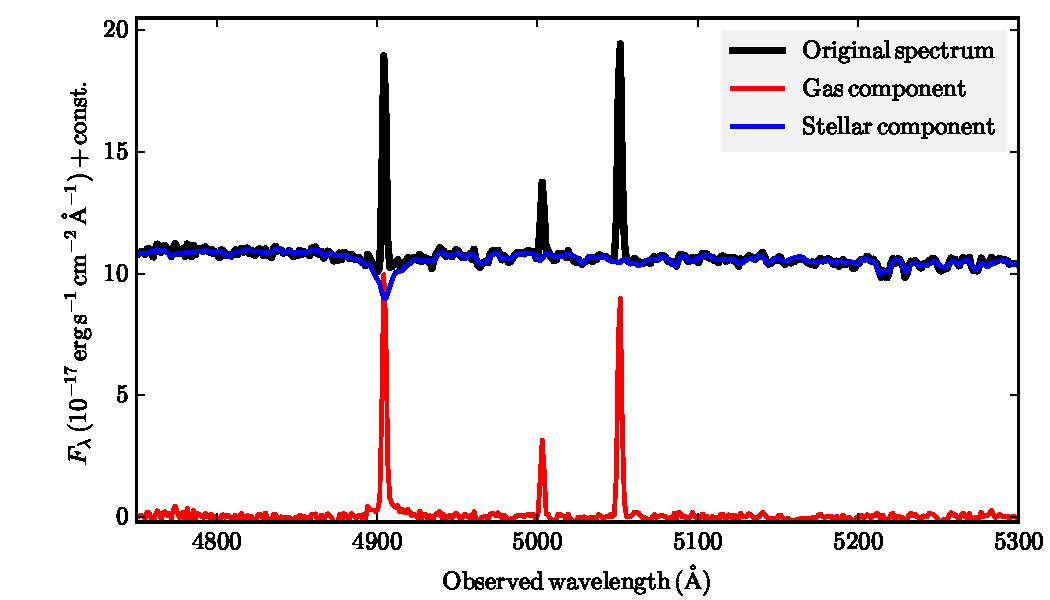
\includegraphics[angle=0, width=0.99\columnwidth]{Figs/Stargas_spec.pdf}
\caption{Separating stellar and gas-phase spectra. This figure shows a zoom-in to the wavelength region around \hb\,including the two strong \oiii($\lambda\lambda4959,5007$) lines at an arbitrary location from the MUSE cube. Black is the original spectrum, blue the fitted stellar component, and red the resulting spectrum for the gas-phase only. Blue and black spectra are shifted to enhance clarity in the Figure. Note the significant Balmer absorption around \hb.}
\label{fig:stargas}
\end{figure}

As we are primarily interested in the absolute and relative strengths of the nebular lines, and thus the gaseous component of the galaxy, we need to remove the stellar component for accurate line flux measurements, in particular for the Balmer lines. The stellar Balmer absorption has a significant influence on the emission line measurement of \hb\, (Figure~\ref{fig:stargas}). It is primarily a function of line intensity and age of the underlying stellar population, and thus depends on the position within a galaxy, and needs to be accurately modeled for reliable constraints on the Balmer decrement.

We separate the galaxy's star and gas components by fitting a linear superposition of template stellar spectra based on the \citet{2003MNRAS.344.1000B} models to the MUSE data. We divide the full field of view into regions with a size of 0\farc{6}x0\farc{6} (or 3 by 3 spaxels), and extract spectra for each of the $\sim9000$ sub-regions. These spectra are then fit with stellar models using \texttt{starlight} \citep{2005MNRAS.358..363C, 2009RMxAC..35..127C} in a similar fashion as we did elsewhere for MUSE data \citep{2016MNRAS.455.4087G, 2016arXiv160703446K, 2016arXiv160900013P}. The 3x3 co-adding effectively is an increase in signal-to-noise at the expense of spatial resolution for the stellar properties, but is necessary to robustly perform an automated fit in particular in the fainter regions of the galaxy. We then linearly scale the best-fit stellar template to the intensity in single spaxels. Subtracting this stellar component from the original data results into the contribution of the gas-phase only (Figure~\ref{fig:stargas}).

\begin{figure}
\begin{center}
  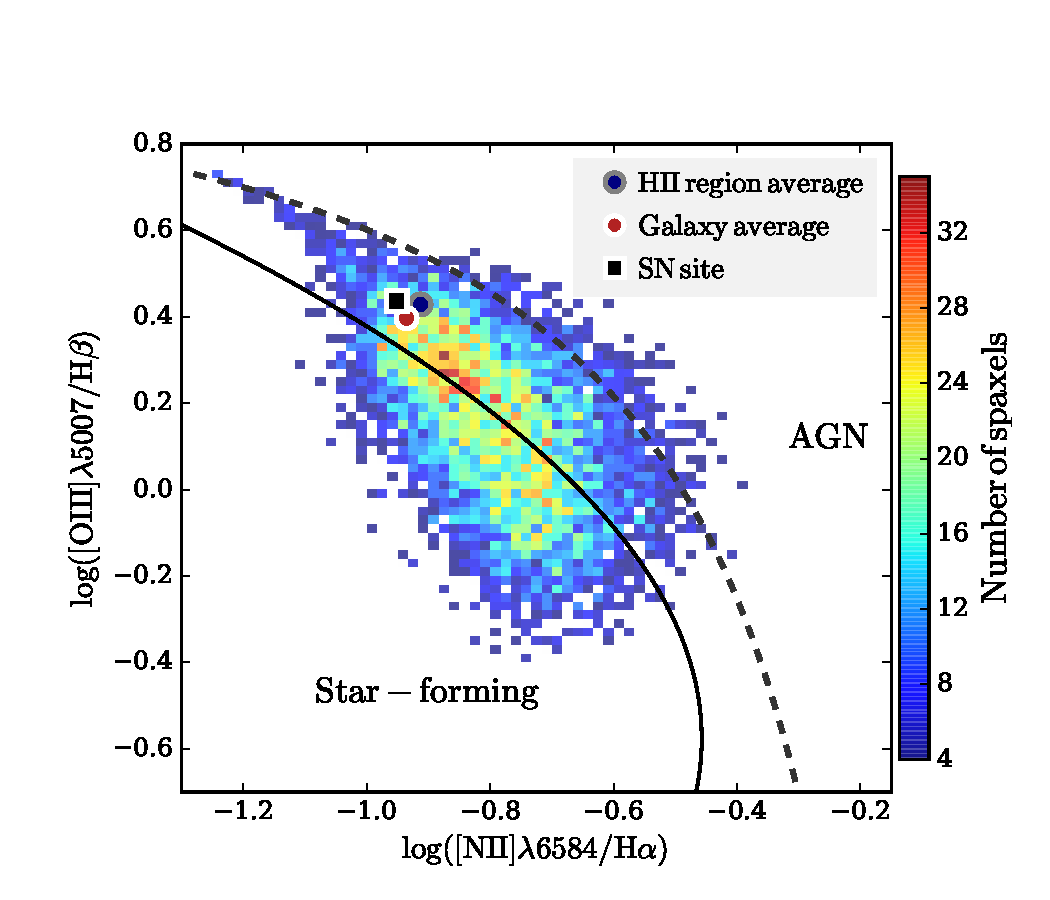
\includegraphics[width=0.75\linewidth]{Figs/MUSE_SN1998bw_BPT.pdf}
\caption{Spaxel BPT diagram for ESO184-G82. The solid line denotes the ridge-line of SDSS galaxies \citep{2008MNRAS.385..769B}, whereas the dotted line represents the $z=0$ classification line between star-formation and AGN as ionization source \citep{2013ApJ...774..100K}. The GRB/SN explosion site value, as well as a galaxy average (including all spaxels) as well as \hii-region average (including only spaxels with EW$_{\mathrm{H\alpha}}>10$\,\AA) are indicated.}
\label{fig:BPT}
\end{center}
\end{figure}


Plotting emission line flux ratios of \oiii/\hb\, versus \nii/\ha\, for individual spaxels in the BPT-diagram \citep{1981PASP...93....5B} allows us to immediately discard active galactic nuclei or shocks as ionization source, and ascertains young stars as origin for the line-emission from ionized gas (Figure~\ref{fig:BPT}).

\subsection{Equivalent Width Maps and Stellar Population Ages}
\begin{figure}
\begin{subfigure}{.242\textwidth}
  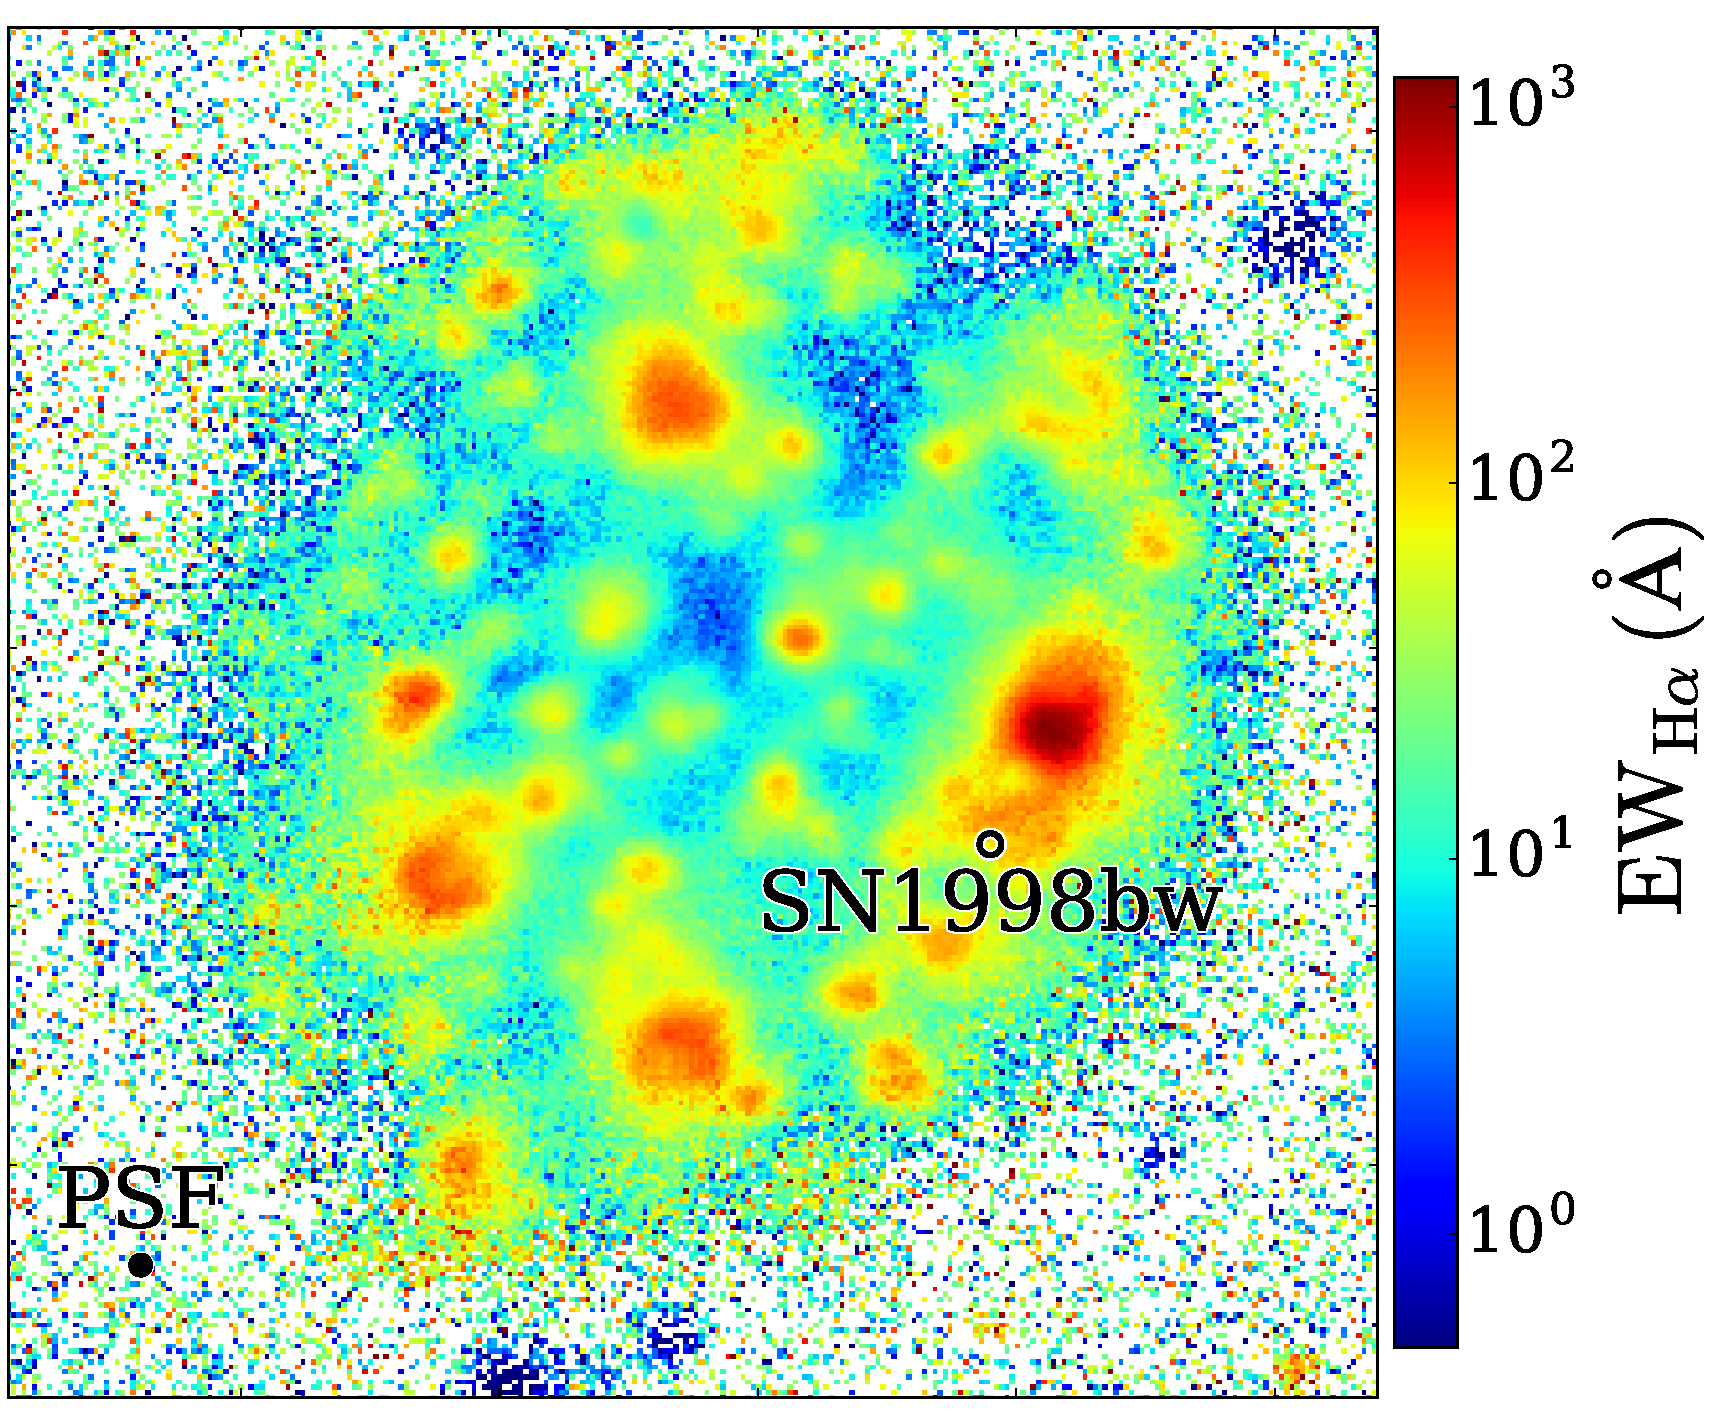
\includegraphics[width=1.0\linewidth]{Figs/MUSE_SN1998bw_HaEW.pdf}
\end{subfigure}
\begin{subfigure}{.242\textwidth}
  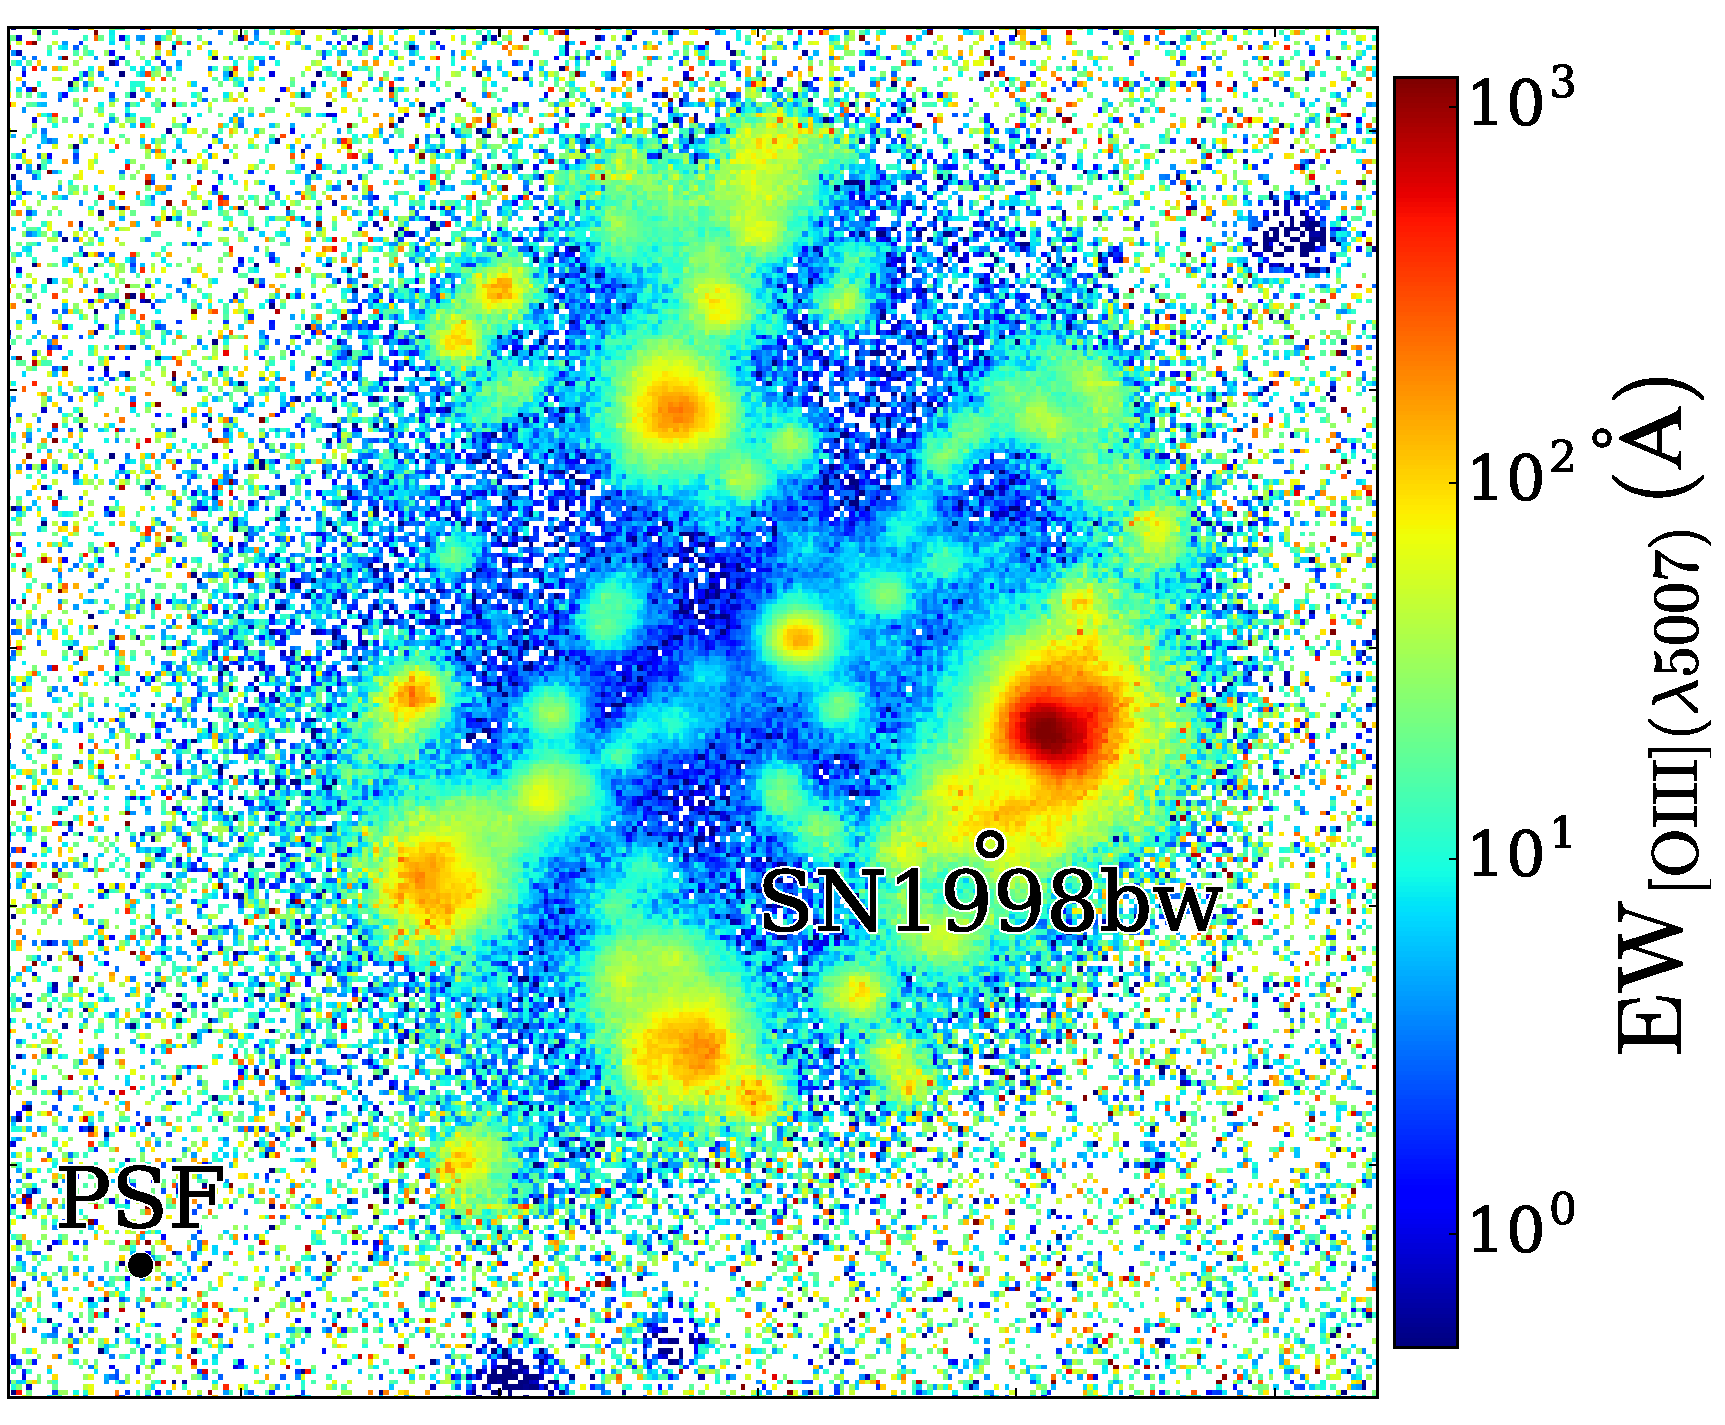
\includegraphics[width=1.0\linewidth]{Figs/MUSE_SN1998bw_OIIIEW.pdf}
\end{subfigure}
\begin{subfigure}{.243\textwidth}
  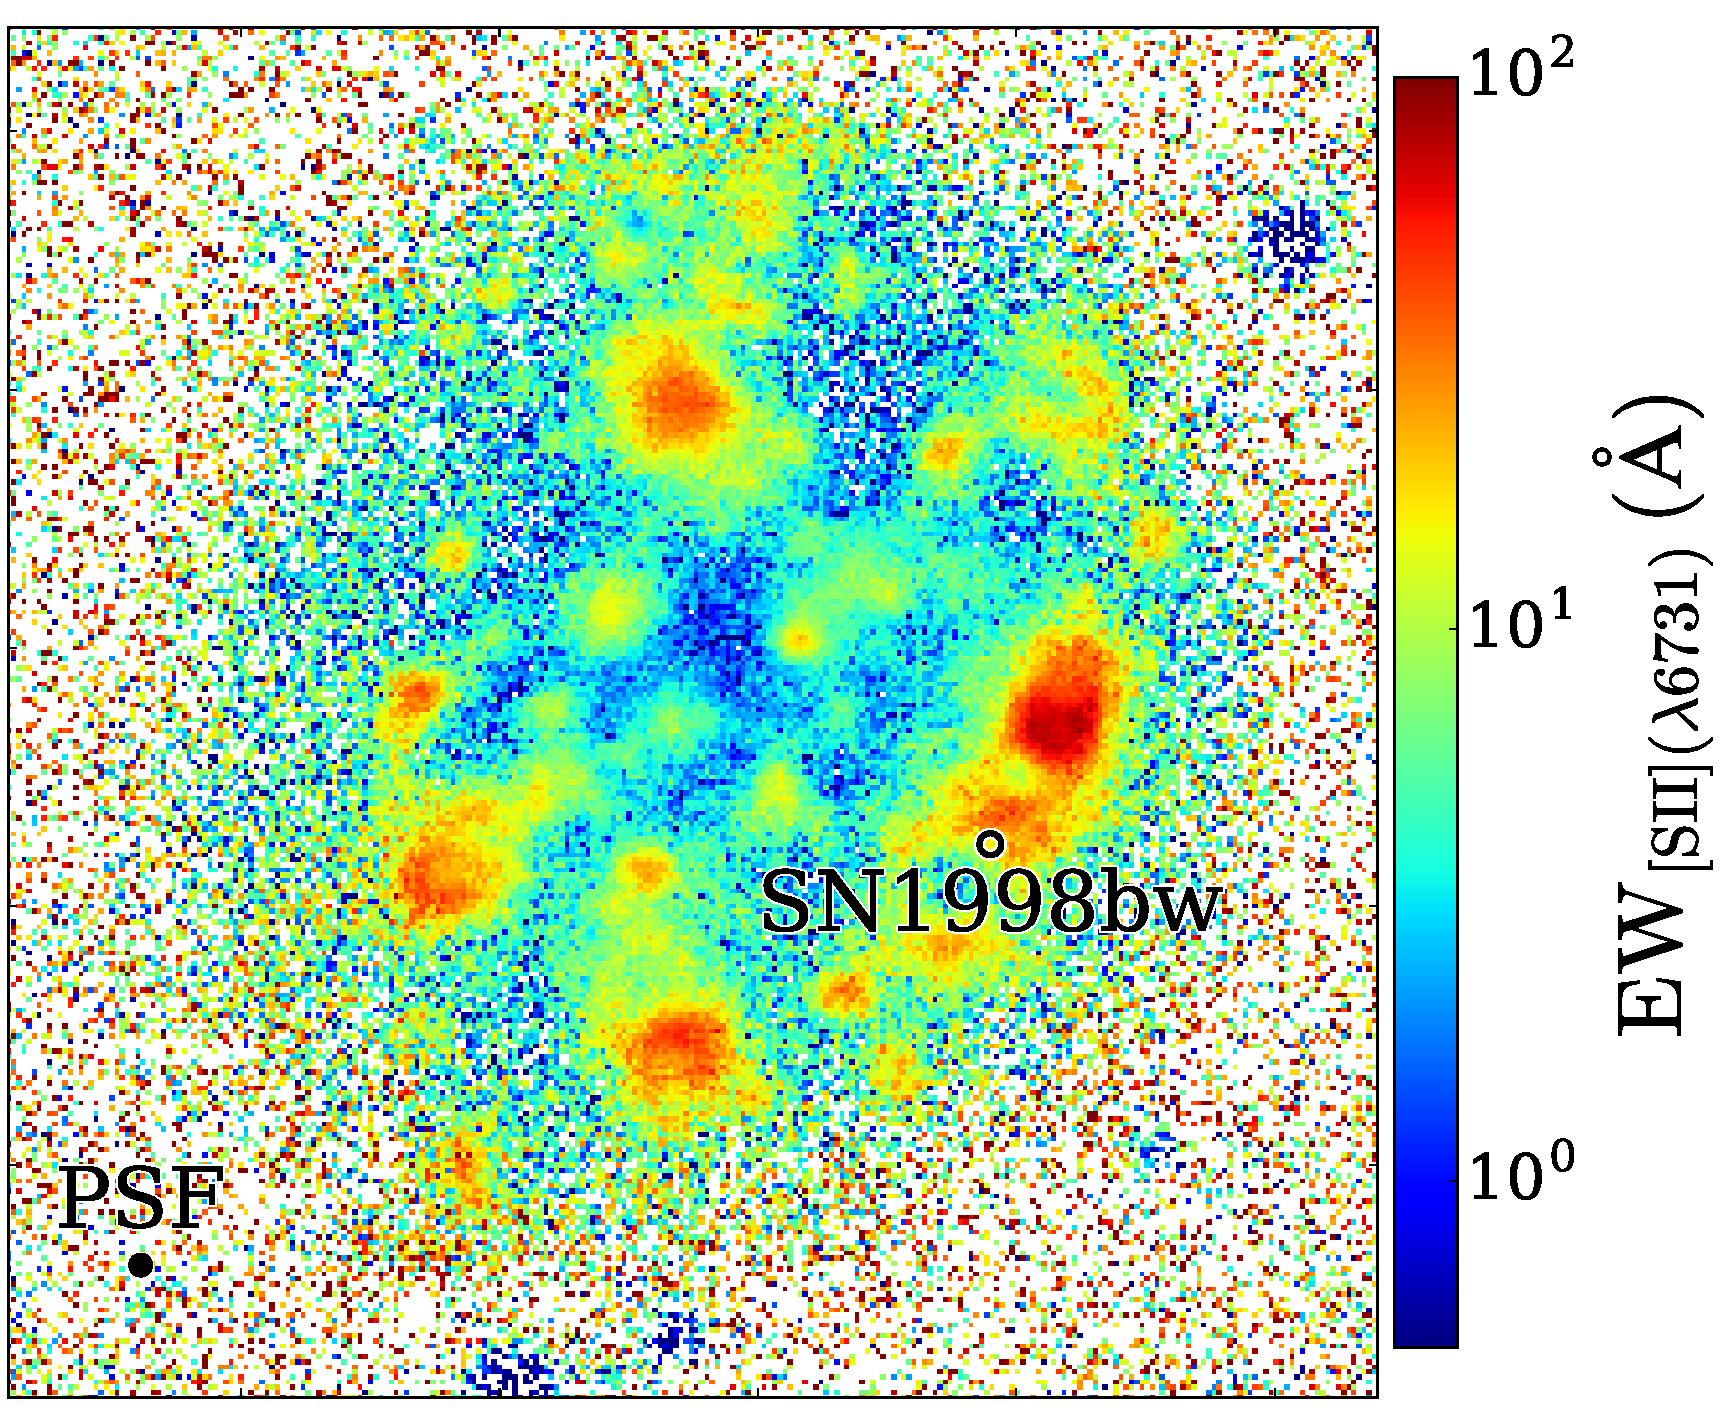
\includegraphics[width=1.0\linewidth]{Figs/MUSE_SN1998bw_SIIEW.pdf}
\end{subfigure}
\begin{subfigure}{.242\textwidth}
  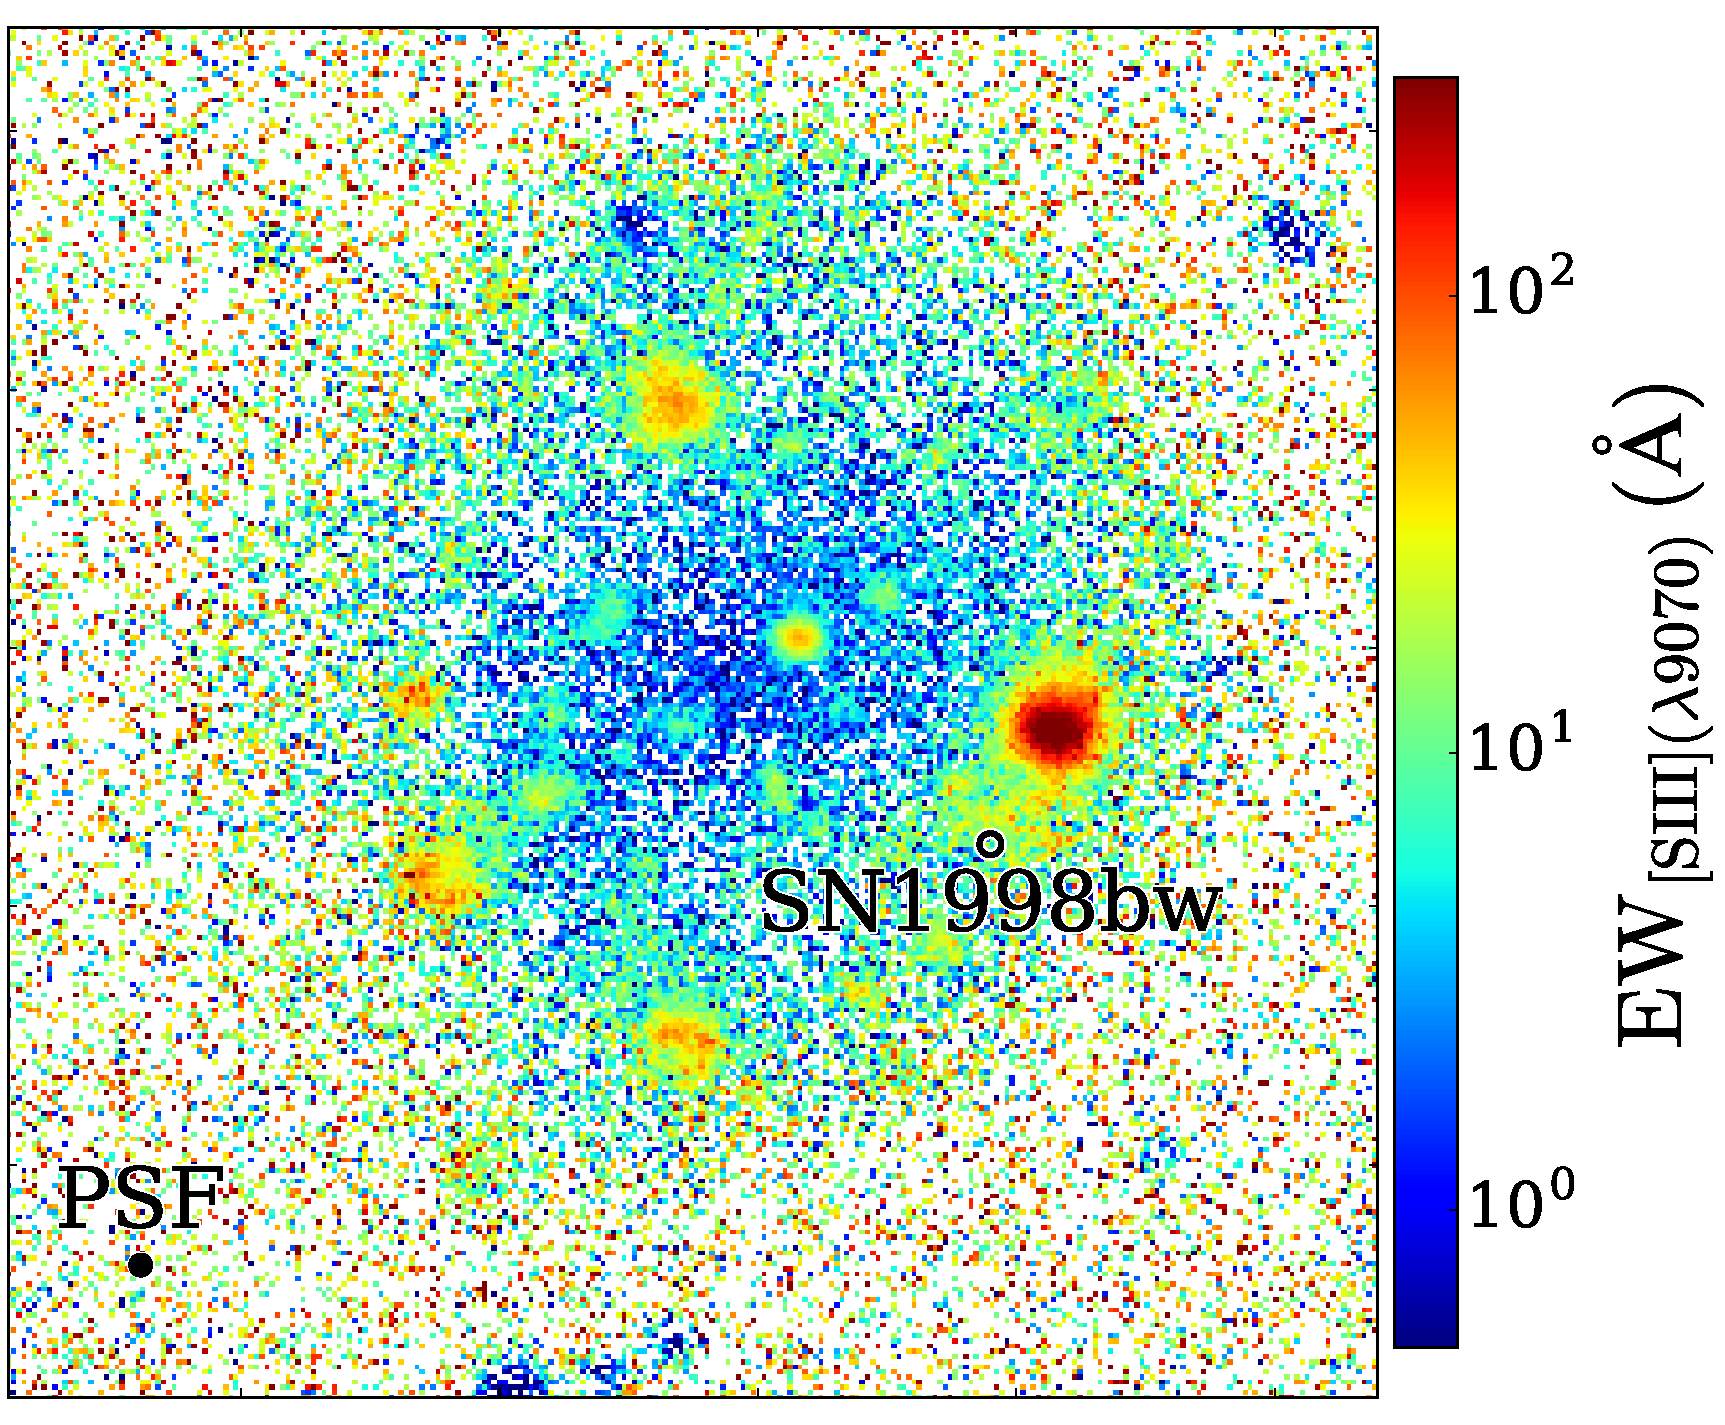
\includegraphics[width=1.0\linewidth]{Figs/MUSE_SN1998bw_SIIIEW.pdf}
\end{subfigure}
\caption{Reconstructed images from the MUSE data cube. Each panel shows the host of GRB~980425 in a different wavelength regime. Top-left: \ha, top-right: \oiii($\lambda$5007), bottom-left: \sii($\lambda$6731), bottom-right: \siii($\lambda$9070). All panels are approximately 55" by 55", or 10 by 10 kpc in size. One MUSE spaxel corresponds to 35~pc. The effective spatial resolution is given by the point spread function indicated in the lower left corner of each image with a FWHM of approximately 0\farc{9}.}
\label{fig:EW}
\end{figure}

After having separated gas-phase and stellar component it is trivial to produce maps of line flux (integral over the gas-phase), continuum (average of the stellar component) and equivalent width (flux over continuum). Figure~\ref{fig:EW}~displays the \ha\,equivalent width map, which is a rather direct proxy of stellar population age, which then can be interpreted as a tracer for progenitor mass. The spaxel closest to the SN/GRB position has an \ha\,equivalent widths of EW=$98\pm4$\,\AA. The spaxels within a radius of 70 pc yield EW$_{\mathrm{H\alpha}}=88\pm15$\,\AA. 

Assuming a single stellar population from an instantaneous starburst, this corresponds to stellar-population ages between 5 Myr and 8 Myrs from various models at metallicities of $Z=0.004$ or $Z=0.2$\,Z$_{\odot}$ \citep[see e.g.][and references therein]{2013ApJ...779..170L, 2016arXiv160703446K}. The relatively large range in ages is almost entirely due to the spread from different stellar evolution models or initial mass functions. These ages corresponds to life-times of stars with zero-age main sequence masses (ZAMS) of approximately 25 to 40~M$_{\odot}$ \citep{1994A&AS..105...29F, 2005A&A...429..581M}. This is consistent with the SN's ejected oxygen mass ($M_{\mathrm{O}}\sim5-6$~M$_{\odot}$ evolved from a $M_{\rm{ZAMS}} \sim 30-35$\,M$_{\odot}$ star) derived through modeling the SN\,1998bw nebular spectra  \citep{2001ApJ...559.1047M, 2006ApJ...640..854M}.

These considerations are only valid, of course, if the progenitor was born where it exploded, and was not ejected from the nearby WR region \citep{2006A&A...454..103H}. However, the WR region is so young such that timing arguments make this scenario very contrived: Very high EW values of \ha~and nebular transitions are observed in the center of the WR-region (both EW$_{\mathrm{H\alpha}}$ and EW$_{\oiii(\lambda5007)}>1000\,\AA)$\footnote{These are strictly lower limits. The fact that the compact WR-region is convolved with the seeing-introduced spatial scale of $\sim$0\farc{9} leads to a smoothed EW distribution. In fact, the FORS2 data discussed in the Appendix were taken under significantly better atmospheric conditions and show EW$_{\oiii(\lambda5007)}\sim2000$\,\AA\,(Sect.~\ref{app:fors}).}. Together with the detection of strong \hei($\lambda4922$), they ascertain population ages younger than 3 Myr (see also Sect.~\ref{app:fors}) in instantaneous star-burst models, or $M_{\mathrm{ZAMS}} \gtrsim 60$\,M$_{\odot}$ \citep[see e.g.][and references therein]{2015MNRAS.451L..65T}. The discrepancy with respect to the progenitor mass from SN modeling then suggests, that the GRB progenitor was indeed not born in the WR-region, but rather formed in situ. 

For the progenitor to travel to the explosion site in less than the age of the WR region ($<3$\,Myr), the required peculiar velocities $v$ are extremely high ($v>260\,\mathrm{km\,s^{-1}}$). This is a strict lower limit, as projection effects further increase the required velocities. Scenarios that are believed to give rise to these kind of massive runaway stars are dynamical few-body encounters or binary supernovae, but both seem unfeasible here: A dynamical ejection produces hyper-velocity stars in only very rare and extreme cases \citep{2001A&A...365...49H, 2012ApJ...751..133P}, and the probability of potential GRB progenitors ($M_{\rm{ZAMS}}\gtrsim 20\,M_\odot$) getting velocity kicks with $>200\,\mathrm{km\,s^{-1}}$ from a companion SN is also practically zero \citep{2011MNRAS.414.3501E}. This makes a binary supernova origin highly implausible as there simply would not be enough time to evolve and explode the primary and eject the secondary to a distance $\gtrsim860$\,pc. Also the fraction of stars ejected by dynamical encounters is of course a function of the elapsed time after star burst, and reaches only 0.01/0.03 at 1 or 3 Myr at $M_{\rm{ZAMS}}\sim 35\,M_\odot$ \citep{2012ApJ...746...15B}, again leaving little time for the ejected star to travel as far as 860 pc (or further).

Given the presence of massive stars in the vicinity of the SN position \citep{2000ApJ...542L..89F}, the substantial level of recent star-formation as evidenced through high EW of nebular lines at the SN position (Figure~\ref{fig:EW}), and the consistency between $M_{\rm{ZAMS}}$ derived from the age of the stellar population as well as the SN~1998bw nebular spectra, we see no compelling reason to invoke an artificial ejection from the nearby \hii-region region to explain the GRB location within its host.

\subsection{Dust Distribution}

\begin{figure}
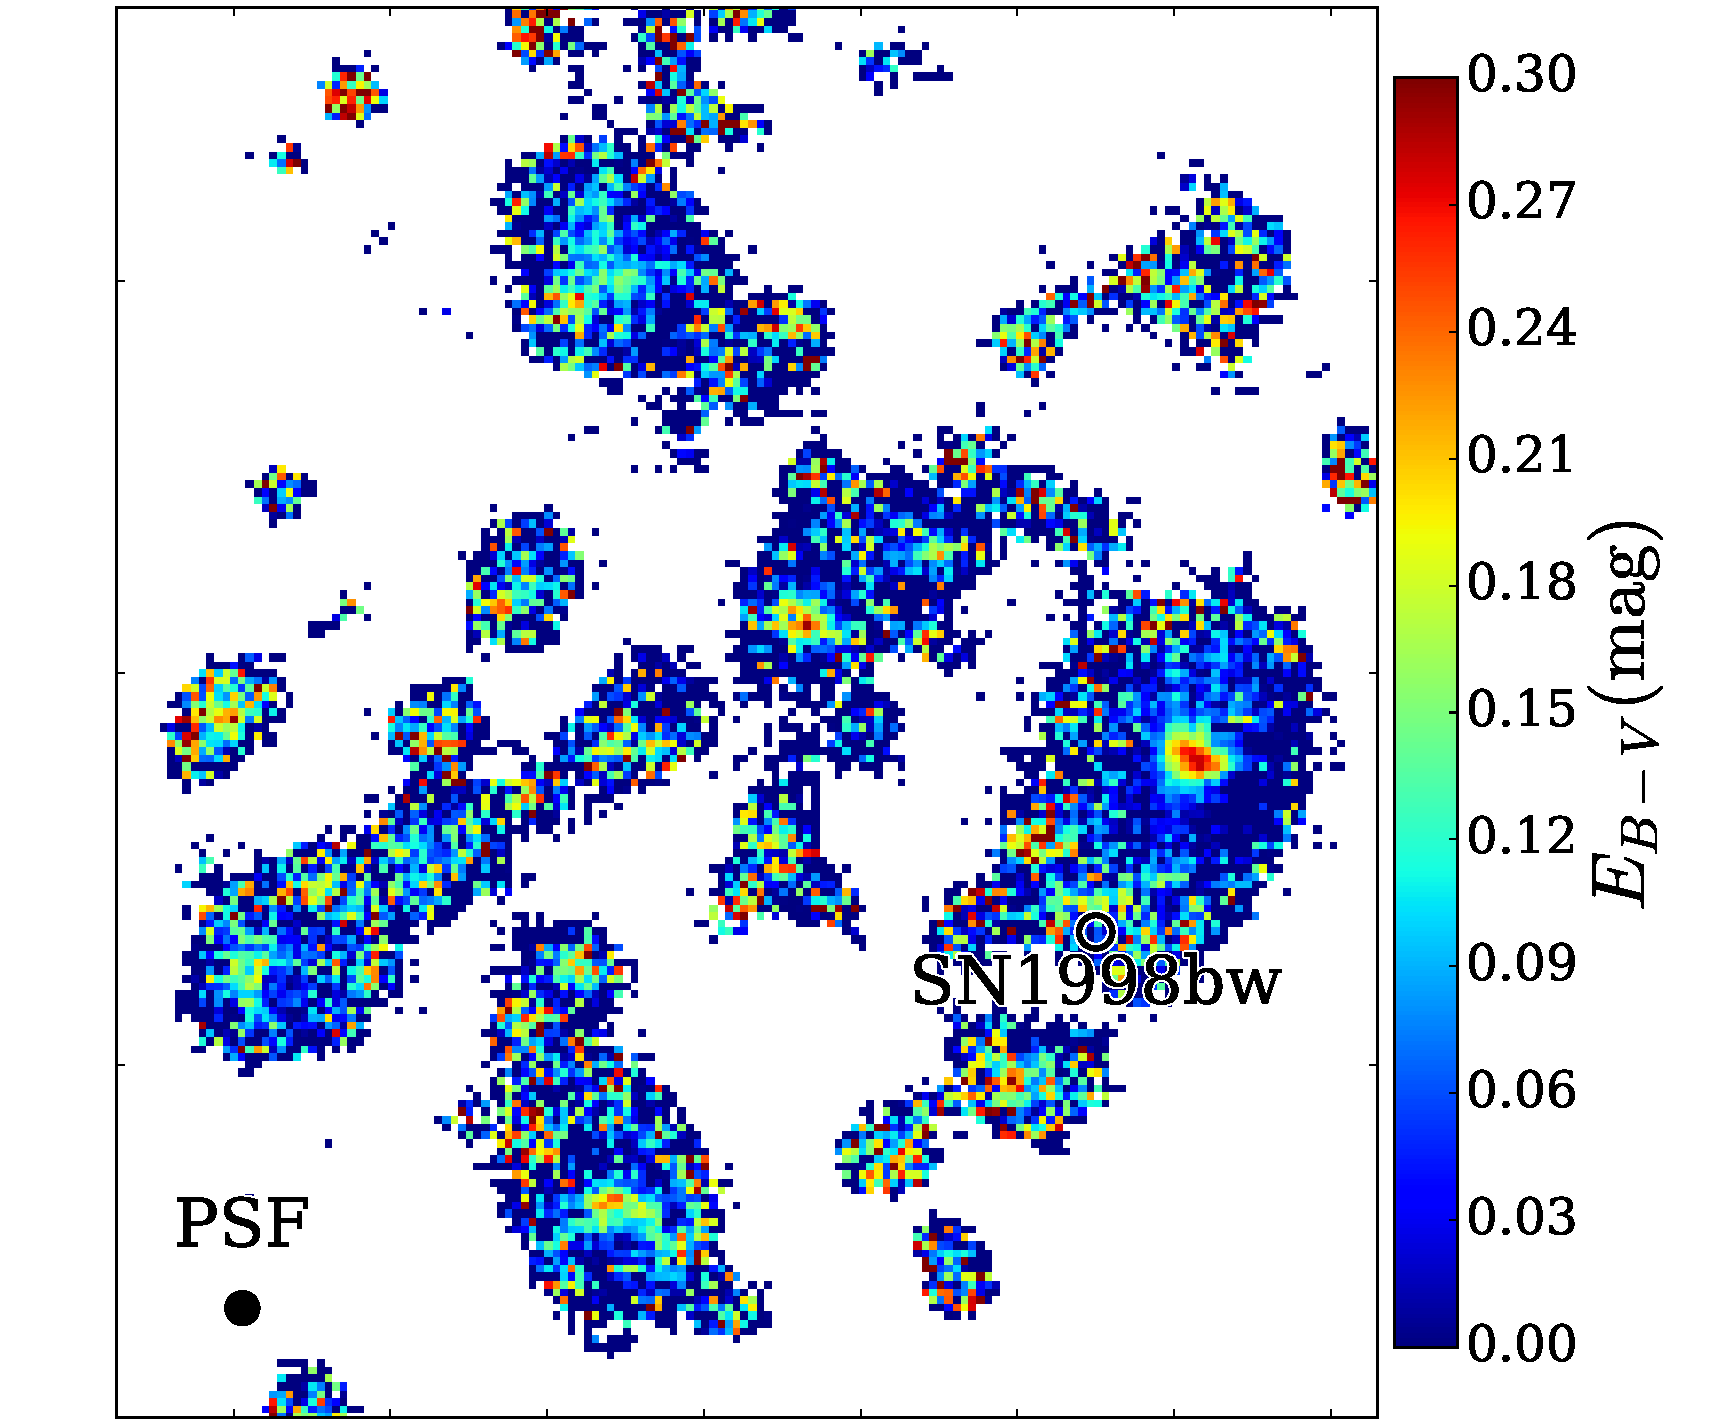
\includegraphics[angle=0, width=0.99\columnwidth]{Figs/MUSE_SN1998bw_EB-V.pdf}
\caption{Dust distribution in ESO184-G82 as measured through the Balmer decrement. We only show spaxels in which \hb\, is detected with a significance of at least 3~$\sigma$. The shown image spans 34" by 38", or 6.1 by 6.8 kpc. The circle denoting the position of SN\,1998bw has a radius of 180 pc.}
\label{fig:ebv}
\end{figure}

Due to its exquisite photometric and spectroscopic data set, SN1998\,bw is a widely-used comparison object, so it is fundamental to quantify the absorbing dust along the line of sight to derive its intrinsic properties. To this end, we convert our line fluxes of \ha\,and \hb\, into a map of color-excess $E_{B-V}$ as shown in Figure~\ref{fig:ebv} using Equation 5 of \citet{2015A&A...581A.125K}. This procedure assumes standard ratios of the Balmer lines at $10^4$\,K and $n_e\sim100\,\mathrm{cm}^{-3}$ from \citet{1989agna.book.....O}, broadly consistent with the values obtained for this galaxy (Table~\ref{tab:prop}). Our results depend only marginally on our choice of an average Milky-Way extinction law \citep{1992ApJ...395..130P} with $R_V=3.08$, as the difference between reddening laws in the local group is small in the wavelength range probed by \ha\, and \hb. 

Figure~\ref{fig:ebv}~shows very little dust in general in ESO184-G82, and also only minor evidence for dust at the actual GRB/SN position ($E_{B-V} = 0.06\,\mathrm{mag}$, or $A_V = 0.19\,\mathrm{mag}$) and its immediate environment $E_{B-V} = 0.03_{-0.03}^{+0.06}\,\mathrm{mag}$ in the 9 spaxels closest to the GRB/SN position). The only location where we observe evidence for significant dust reddening are the centers of \hii\, regions as exemplified by the WR-region. They show a centrally-symmetric substructure in dust extinction decreasing from the inside out peaking at $E_{B-V} \sim 0.25\,\mathrm{mag}$ or $A_V = 0.8\,\mathrm{mag}$. A galaxy-integrated spectrum yields $E_{B-V} = 0.05\pm0.02$~mag, or $A_V=0.15\pm0.06$~mag, which is in remarkable agreement with the average optical depth $\tau_V$ derived from modeling the UV-to-radio SED \citep{2014A&A...562A..70M}.

Our new data thus resolve the apparent conflict with the unexpectedly large reddening at the SN position derived from previous spectroscopic data \citep{2006A&A...454..103H, 2008A&A...490...45C} and the SN itself, which did not show any evidence of strong dust obscuration \citep[e.g.][]{1998Natur.395..672I, 2001ApJ...555..900P}. They provide further confidence in using SN\,1998bw as an only very mildly reddened SN template for comparison to other GRB/SNe \citep[e.g.][and numerous references therein]{2004ApJ...609..952Z, 2016arXiv160606791K}.

\subsection{Metallicity Diagnostics}

\subsubsection{Initial considerations}


Metal abundances in \hii\,regions are a central observable to study cosmo-chemical evolution, and a large set of literature is devoted to the various possibilities, their advantages, and perils to infer abundances from \hii-region spectra  \citep[e.g.][]{1979MNRAS.189...95P, 1991ApJ...380..140M, 2005ApJ...631..231P, 2008ApJ...681.1183K}. Very briefly, the most common methods to infer chemical abundances, and from those, the abundance of oxygen (traditionally expressed in \oh) make use of either photo-ionization models \citep[e.g.][]{1985ApJS...58..125E, 2000ApJ...542..224D, 2002ApJS..142...35K} or empirical correlations between certain strong-line ratios and oxygen abundances derived through electron temperatures $T_{\rm{e}}$ from collisionally-excited lines \citep[CELs, e.g.][]{2004MNRAS.348L..59P, 2013A&A...559A.114M}. Commonly used ratios are for example \nii/\oii, \oiii/\nii, \nii/\ha, or $R_{23}$ = (\oii+\oiii)/\hb, which have been (re)-calibrated numerous times against different samples of $T_{\rm{e}}$ or photo-ionization models, yielding a large set of different calibrators in the literature \citep[e.g.][]{2002ApJS..142...35K, 2004ApJ...617..240K, 2005ApJ...631..231P, 2006A&A...459...85N, 2008A&A...488..463M}.

One of the fundamental problems in using and interpreting the oxygen abundances derived in this way is that different methods are only very rarely consistent \citep[e.g.][]{2008ApJ...681.1183K} giving rise to the abundance determination problem \citep{1967ApJ...150..825P}. Methods based on temperature-sensitive collisionally-excited lines typically show abundances that are lower by 0.2-0.4 dex with respect to photoionization-based methods or abundances derived using temperatures from recombination lines \citep[e.g.][and references therein]{2012MNRAS.426.2630L}, in particular in the high-metallicity region. A possible solution to the abundance determination problem are small-scale temperature fluctuations \citep[e.g.][]{2003ApJ...584..735P, 2004MNRAS.355..229E} or an electron population distributed somewhat differently than in thermal Maxwell-Boltzmann equilibrium \citep{2012ApJ...752..148N, 2012MNRAS.426.2630L}, but until these discrepancies are fully resolved, element abundances from emission lines remain the subject of large controversy.

A second, independent problem relates to the observational difficulties in robustly measuring emission line fluxes for lines in different wavelength ranges for faint, high-redshift galaxies. Due to various observational constraints, the available data is typically limited to a handful of strong lines. This is similarly true for our observations, as the MUSE data do not cover neither the strong \oii($\lambda\lambda3726,3729$)~doublet nor \oiii($\lambda 4363$), one of the most commonly-used, temperature-sensitive CEL. A very popular emission-line diagnostic in the literature has thus been the logarithm of the ratio of \oiii\,/\hb\,to \nii/\ha\, or short O3N2 \citep[e.g.][]{2004MNRAS.348L..59P, 2013A&A...559A.114M}, because of its independence on dust reddening and relative observational ease with which it can be measured even at $z\sim 2$.

\subsubsection{Specific Problems of Empirical Metallicity Diagnostics}

\begin{figure}
\begin{subfigure}{.24\textwidth}
  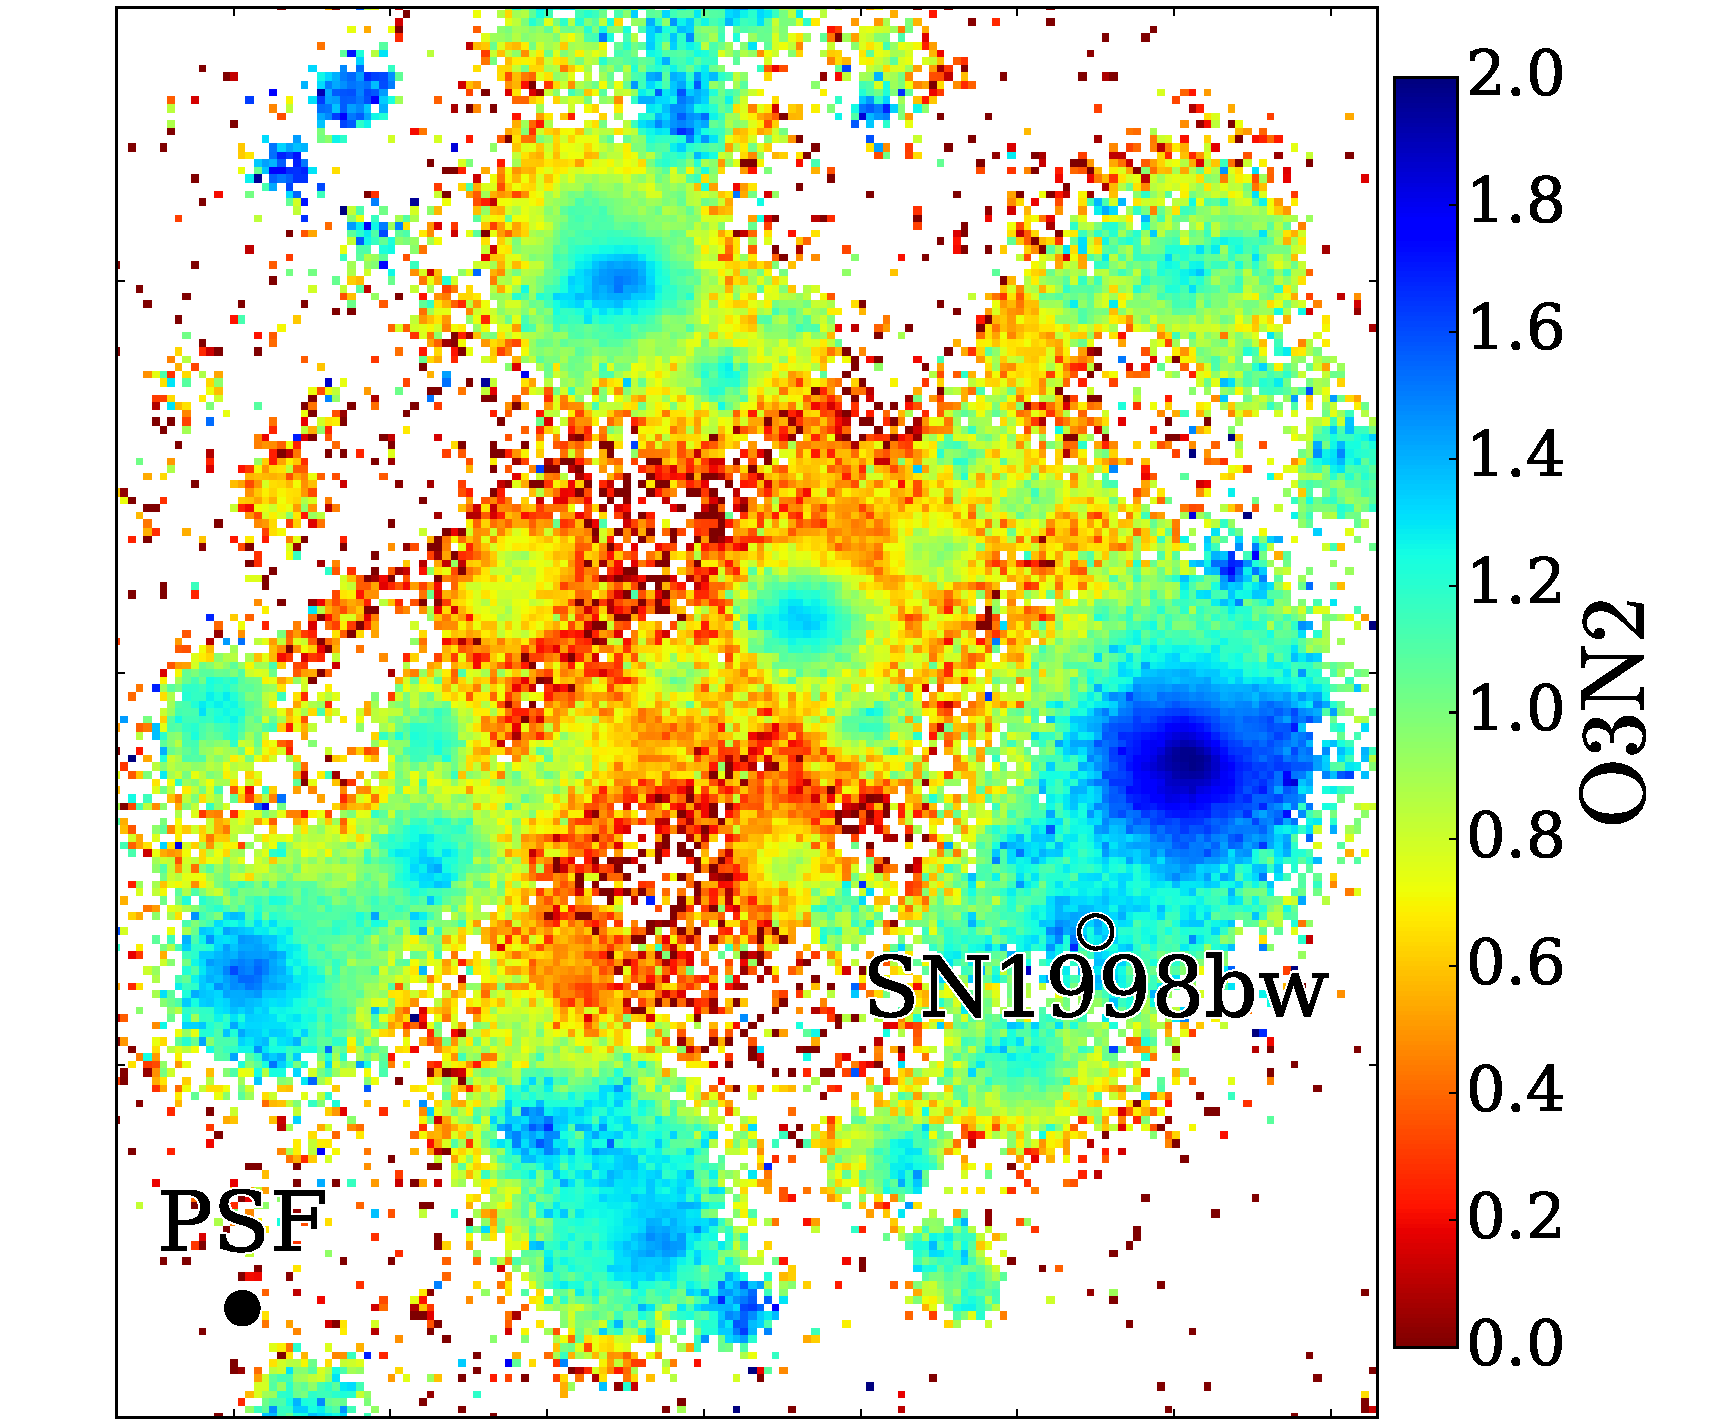
\includegraphics[width=0.999\linewidth]{Figs/MUSE_SN1998bw_O3N2.pdf}
\end{subfigure}
\begin{subfigure}{.24\textwidth}
  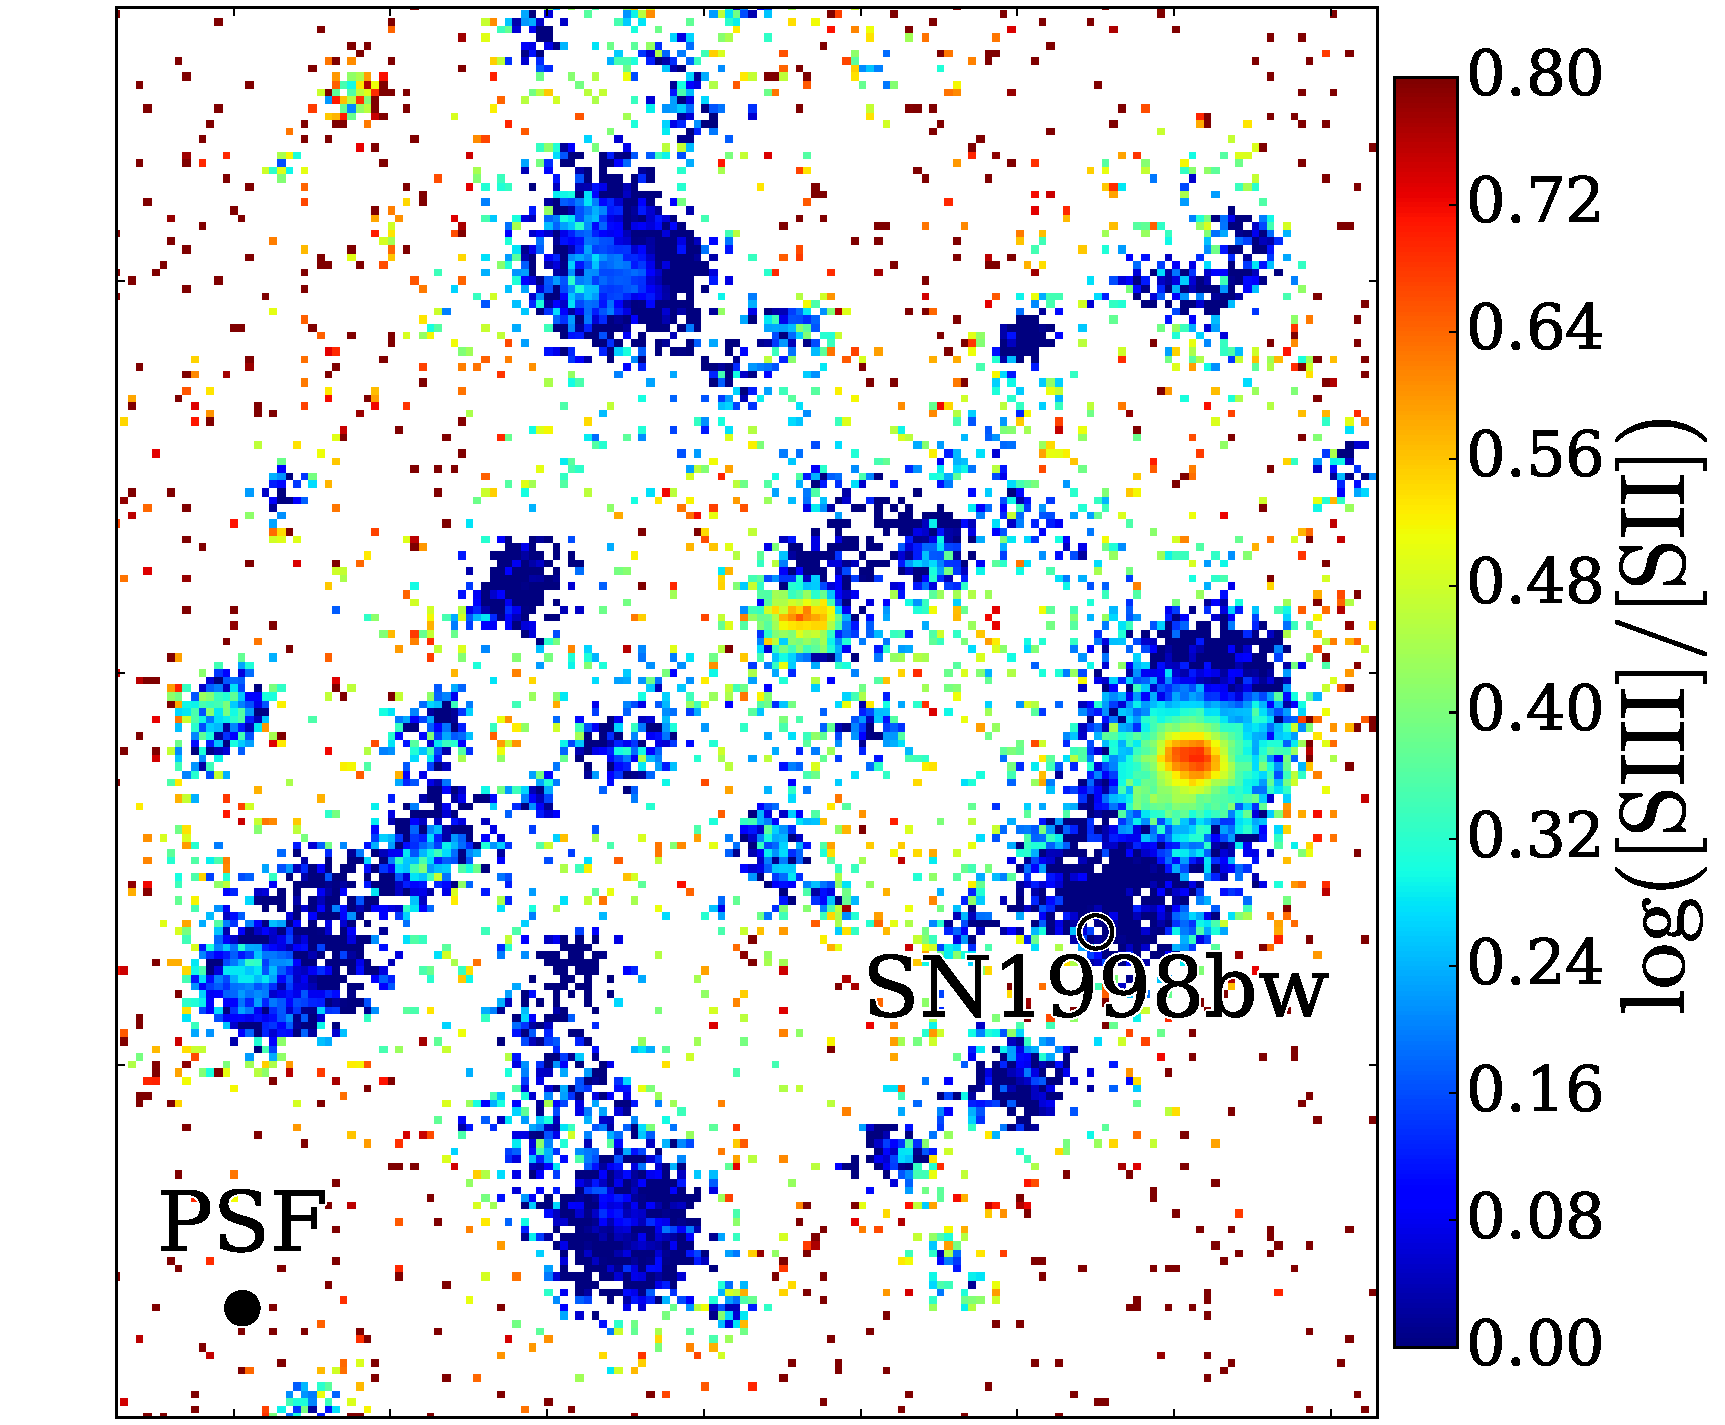
\includegraphics[width=0.999\linewidth]{Figs/MUSE_SN1998bw_S3S2.pdf}
\end{subfigure}
\caption{Face-to-face comparison between the maps of O3N2, often used for abundance determinations and \siii/\sii, a tracer of the ionization state of the hot gas. Only spaxels with SNR > 3 are shown. Image dimensions are similar to Figure~\ref{fig:ebv}.}
\label{fig:s3s2}
\end{figure}

Yet, from the very different ionization potentials of N and O$^{+}$ (14.5~eV versus 35.1~eV), it is immediately clear that O3N2 also carries a strong dependence on the ionization parameter in addition its inverse proportionality with oxygen abundance \citep[e.g.][]{1979A&A....78..200A, 2015MNRAS.448.2030H}. In Figure~\ref{fig:s3s2}, we plot the O3N2 map, which would immediately translate into a map of oxygen abundance, (\oh\,would be lowest were O3N2 is highest) in common diagnostics \citep{2004MNRAS.348L..59P}.

However, when inspecting the left part of Figure~\ref{fig:s3s2} it becomes apparent that O3N2-based oxygen abundances  (and similarly for those based on N2) would produce abundance maps that are hard to explain in a physical context: O3N2 varies significantly on $\lesssim$ kpc scales, and would lead to an unexpected\footnote{Despite the filamentary structure of nearby giant \hii~regions like 30 Doradus, they are usually adequately described with abundances that are homogeneous throughout the region \citep[e.g.][and references therein]{2011ApJ...738...34P}.}, chemically inhomogeneous structure within individual \hii~regions with their central abundances up to 0.3 dex lower than their outer edges. However, we believe that the significant gradients in O3N2/N2 observed in most of our \hii~regions are unlikely due to a genuine gradient in oxygen abundance but more likely the effect of a changing ionization parameter on O3N2/N2. We will explore this hypothesis further in the following sections.

\subsubsection{Ionization Maps}

Our MUSE data is of sufficient depth and quality to test how strongly O3N2 is affected by ionization empirically through the ratio of \siii\,(IP=23.3~eV) to \sii\,(IP=10.3~eV), widely considered as one of the best tracers of the ionization parameter \citep{1991MNRAS.253..245D} as it shows in contrast to \oiii/\oii\,only very little dependence on abundance itself \citep{2002ApJS..142...35K, 2011MNRAS.415.3616D}. The resulting map\footnote{As MUSE does not cover the wavelength range of \siii($\lambda$9532), we use a theoretical value of $\siii(\lambda9532)=2.44\times\siii(\lambda9069)$ \citep{1982MNRAS.199.1025M} here.} is shown in Figure~\ref{fig:s3s2} and clearly highlights the \hii~region centers standing out with the largest values of \siii, and thus ionization parameter. 

This adds further support to our initial conjecture, and attributes the radial symmetric structure of individual \hii-regions in the O3N2 and N2 maps to an increase of the ionization parameter towards the center of \hii~regions and not chemical inhomogenities. Simple O3N2, or N2-based diagnostic are thus inadequate to produce accurate maps of oxygen abundance at the level of detail of our MUSE data (see also Sect.~\ref{sec:abundancevsion}).

\subsubsection{Metallicity Maps}
\label{sec:mapoh}

\begin{figure}
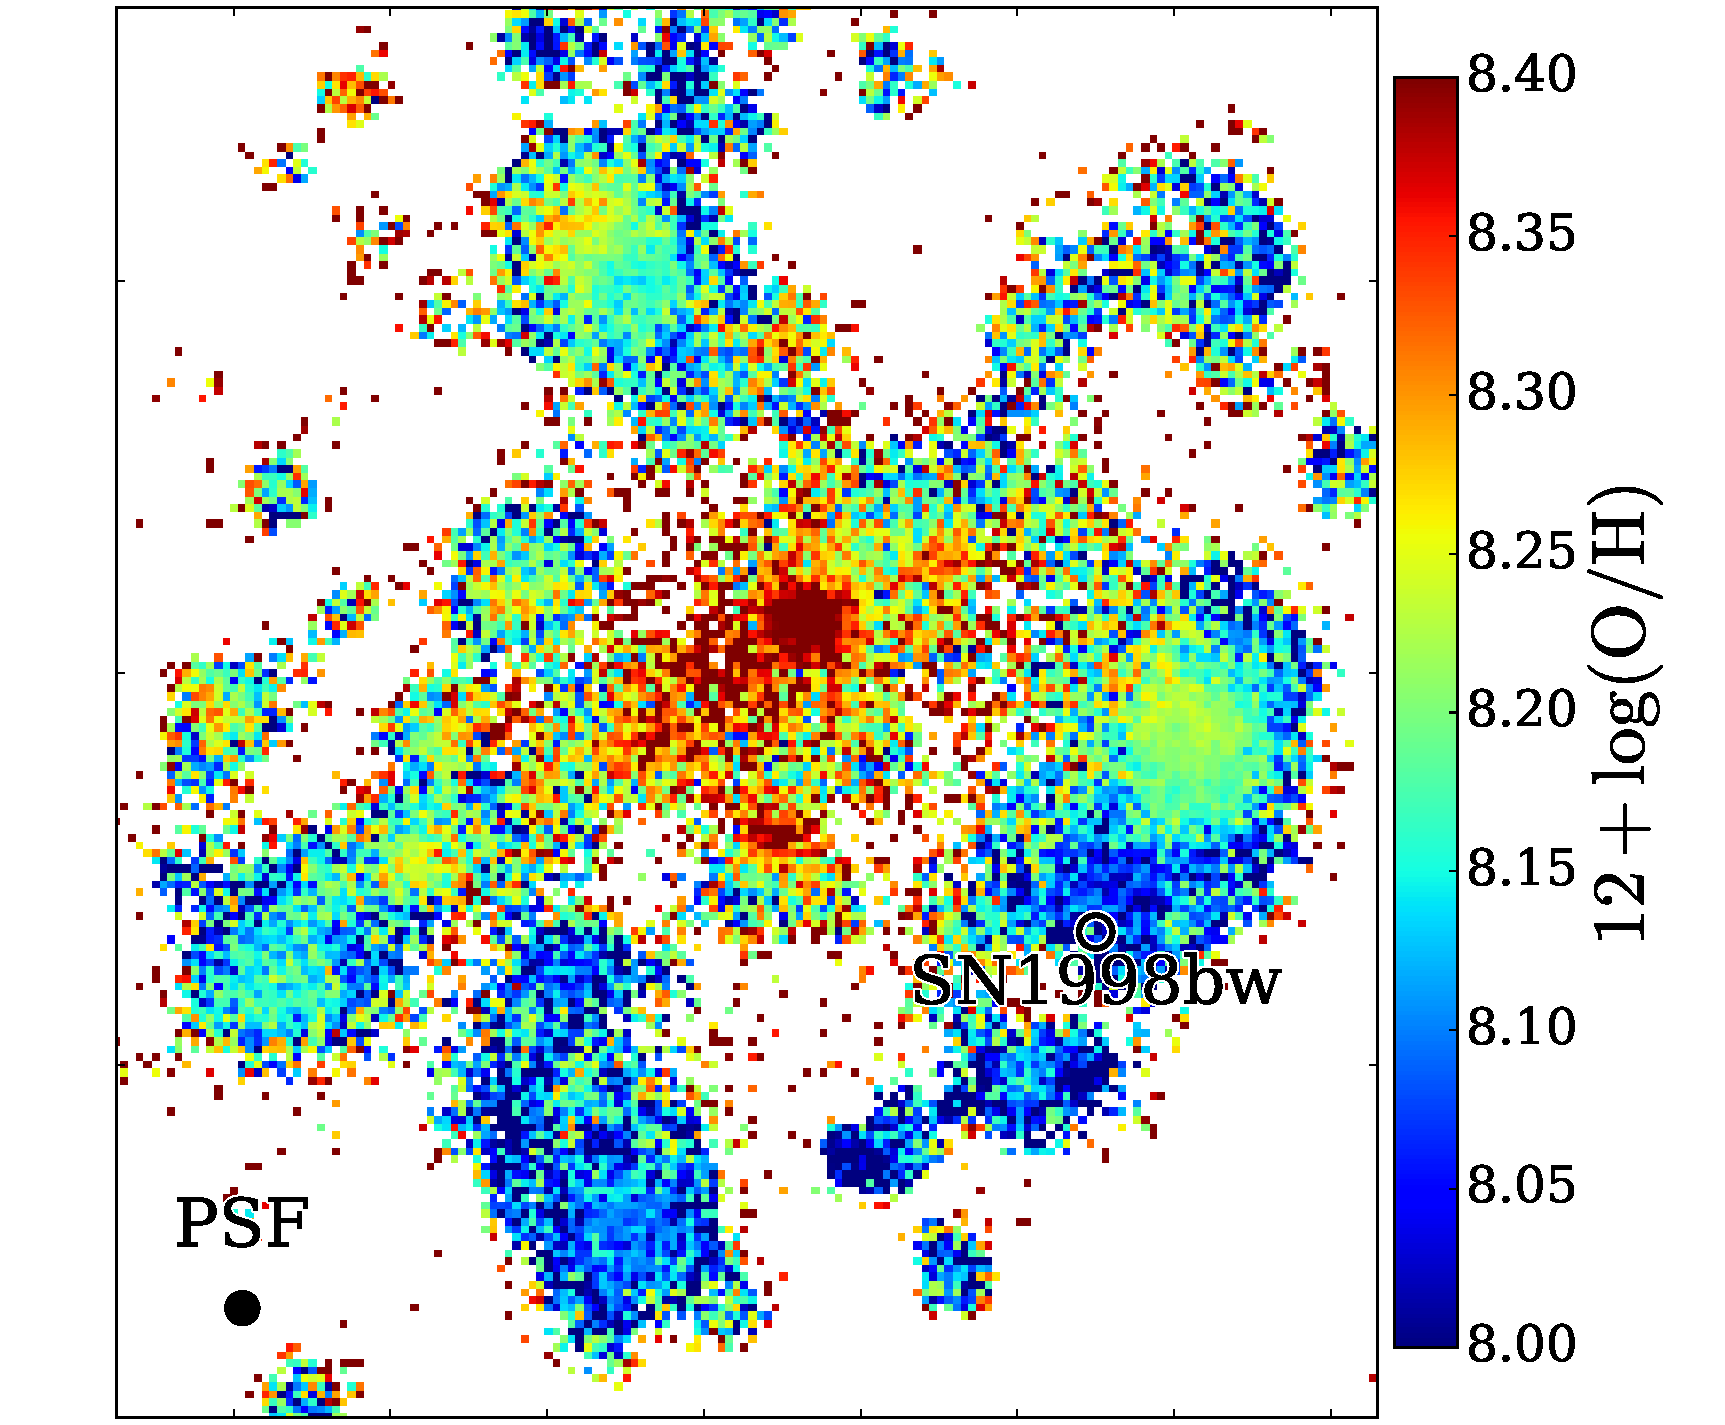
\includegraphics[angle=0, width=0.99\columnwidth]{Figs/MUSE_SN1998bw_OH.pdf}
\caption{Map of \oh\, as obtained through the \sii\, and \nii\, based calibration of \citet{2016Ap&SS.361...61D}. Only spaxels with SNR > 3 are shown. Image dimensions are 34" by 38", or 6.1~kpc by 6.8~kpc, similar to Figure~\ref{fig:ebv}. The circle denoting the position of SN\,1998bw has a radius of 180 pc. Abundance determination methods via lines that are sensitive to electron temperature return 0.1-0.2 dex values.}
\label{fig:s2}
\end{figure}

After rejecting common empirical methods using O3N2 or N2 as reliable metallicity tracer due to their ionization dependence, we turn to diagnostics based on photo-ionization models. Unfortunately, most of the previous strong-line methods rely in one way or another on the strong \oii($\lambda\lambda$3726,3729)\, doublet\citep{2002ApJS..142...35K}, which is not directly available to us here. Also \siii/\sii\, is a good ionization tracer, but \siii\,is relatively faint and not detected in most of our spaxels (see Figure~\ref{fig:s3s2}). A recently published method based on photo-ionization modeling \citep{2016Ap&SS.361...61D} seems to perfectly fit to our data: it relies solely on \ha, \nii, and \sii, which are all strong and well within the wavelength range of MUSE. The method is introduced as "effectively independent of both ionization parameter and ISM pressure" \citep{2016Ap&SS.361...61D}, and Figure~\ref{fig:s2} displays the respective map of \oh\, in regions where all necessary lines are detected at a signal-to-noise ratio of at least 5.

Clearly, the strong abundance gradient over individual \hii-regions as would have been deduced from O3N2, is not observed in this diagnostic. Instead, the oxygen abundance map displays a relatively smooth behavior with a decreasing overall metallicity from the center of the galaxy towards the outside (see also Sect. \ref{sec:metgrad}). The spaxel abundance at the SN position is \oh=8.00 or 0.20\,Z$_{\odot}$. The immediate environment is consistent with this value and homogeneous: within a radius of 70 pc to the SN position \oh is $8.06\pm 0.06$. The WR region displays a somewhat higher metallicities with the oxygen abundances of at the peak of the \ha\,emission yielding \oh$=8.21\pm 0.03$ or $0.33\pm0.03\,$Z$_{\odot}$.

It is of course reasonable to ask now whether the new \citet{2016Ap&SS.361...61D} diagnostic provides more reliable constraints on oxygen abundance than previous methods given the significant differences that exists between all of them \citep{2016arXiv161108595B}. In addition, for low-mass galaxies as is the case here, this diagnostic seems to return lower oxygen abundances than previous methods \citep{2016ApJ...823L..24K}. To elaborate further on the \sii-based diagnostic, we reproduce the combined Equation 1 and 2 from \citet{2016Ap&SS.361...61D}

\begin{equation}
12+\log(\mathrm{O/H}) = 8.77 + \log([\ion{N}{ii}]/[\ion{S}{ii}]) + 0.264\log([\ion{N}{ii}]/\mathrm{H}\alpha)
\end{equation}

with \nii\, being the flux in the \nii($\lambda6484$) line, and \sii\, the flux in the \sii($\lambda\lambda6717,6731$) doublet. The primary observable is thus the nitrogen to sulfur ratio, which is a tracer of the nitrogen to oxygen ratio\footnote{Sulfur and oxygen are both $\alpha$-process elements produced in massive stars, and observed to track each other well in different environments \citep[see e.g. Figure 6 in][]{2006A&A...448..955I}.}. Because nitrogen is also produced in intermediate mass stars, N/O starts to depend on \oh\,above \oh$\sim 7.8$ \citep[e.g.][]{1999ApJ...511..639I, 2013A&A...549A..25P, 2016A&A...595A..62P}, and as expected, a N/O map via \citet{2010ApJ...715L.128A} is very similar to the map of oxygen abundance in the respective strong line diagnostic. 

The map of oxygen abundance then fundamentally relies on the N/O-to-O/H, calibration, and it is in principle not impossible that the applied calibration is somewhat offset, in particular in the low-metallicity region. There could also be internal variations in N/O at a given \oh, or differences between the host of SN\,1998bw to the calibration sample. For example infall of primordial gas would decrease \oh, but leave N/O unaffected \citep{2016ApJ...823L..24K}. Another point of concern would be an anomalously high N/O ratio for the SN region as claimed in \citet{2006A&A...454..103H}. However, both of these effects would lead us to over predict the actual oxygen abundance in the SN region, whereas we observe some of the lowest values here. Also the calibration sample for N/O-to-O/H in the metallicity range of interest is based on low-metallicity blue compact dwarf galaxies \citep{1999ApJ...511..639I}, not dissimilar in physical properties to our galaxies. 
\subsubsection{Metallicities Based on Electron Temperatures}

\begin{figure}
\begin{subfigure}{.242\textwidth}
  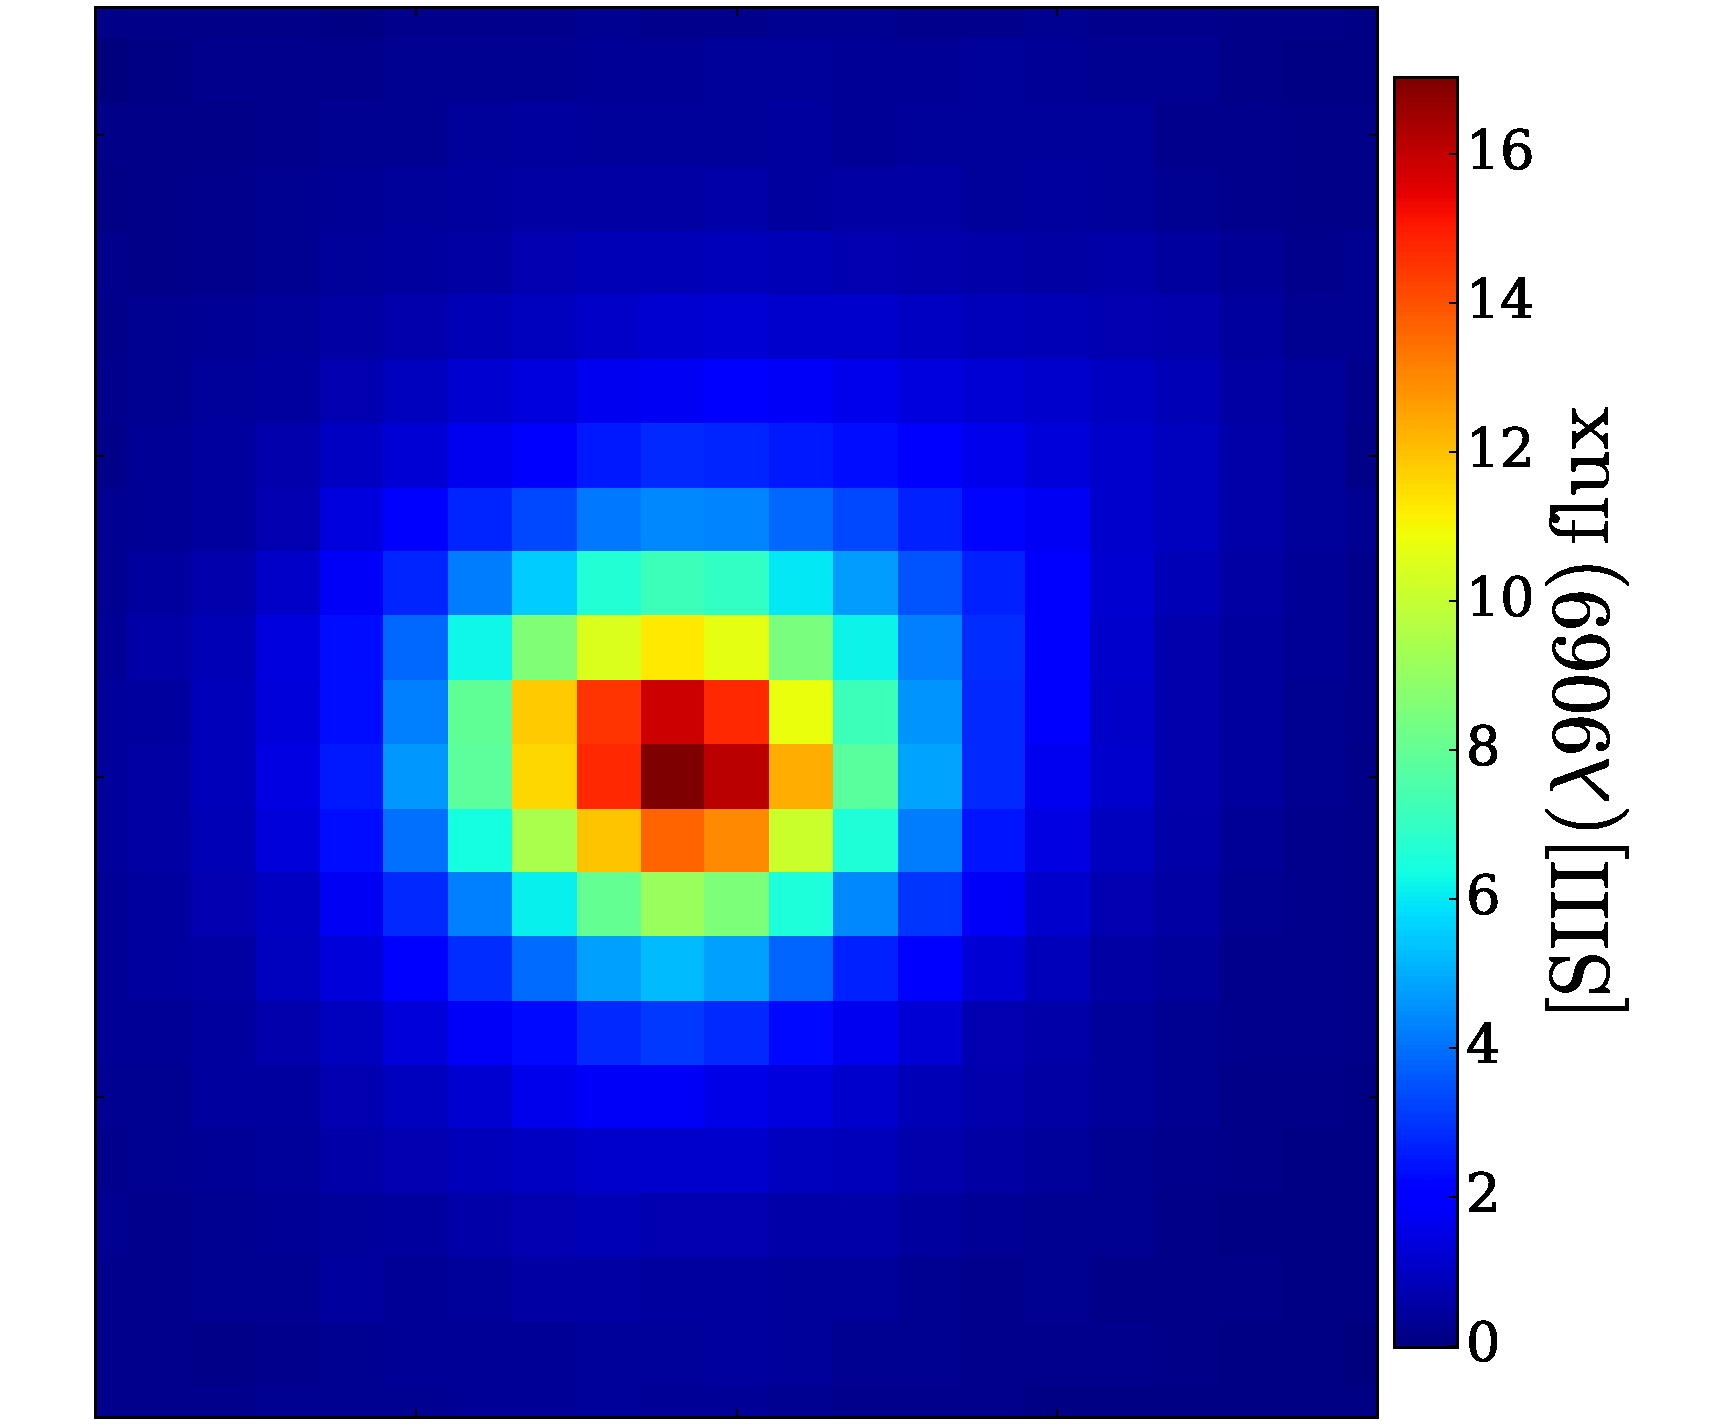
\includegraphics[width=0.999\linewidth]{Figs/MUSE_SN1998bw_SIIIzoom.pdf}
\end{subfigure}
\begin{subfigure}{.242\textwidth}
  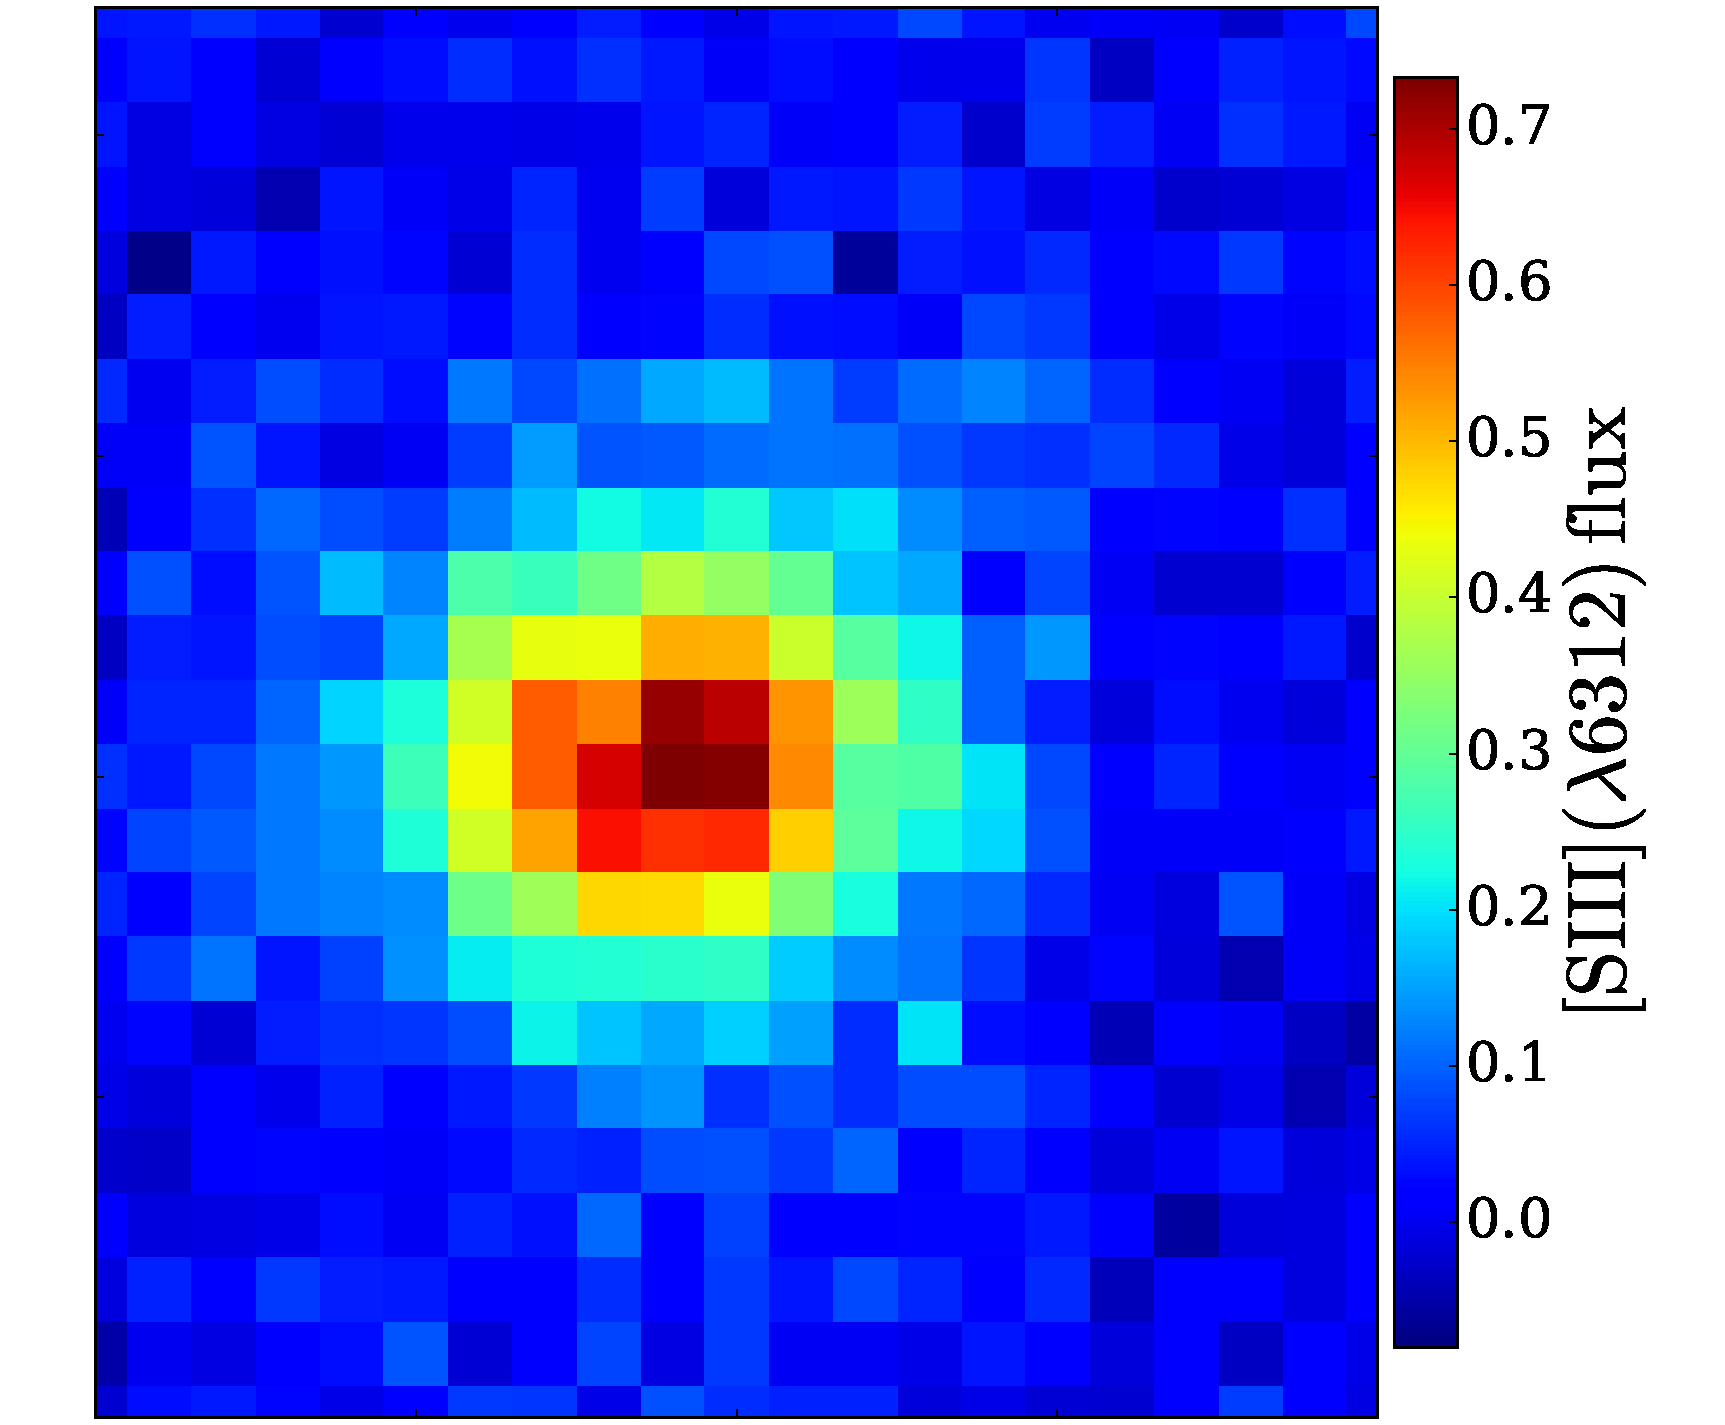
\includegraphics[width=0.999\linewidth]{Figs/MUSE_SN1998bw_SIIIauzoom.pdf}
\end{subfigure}
\begin{subfigure}{.243\textwidth}
  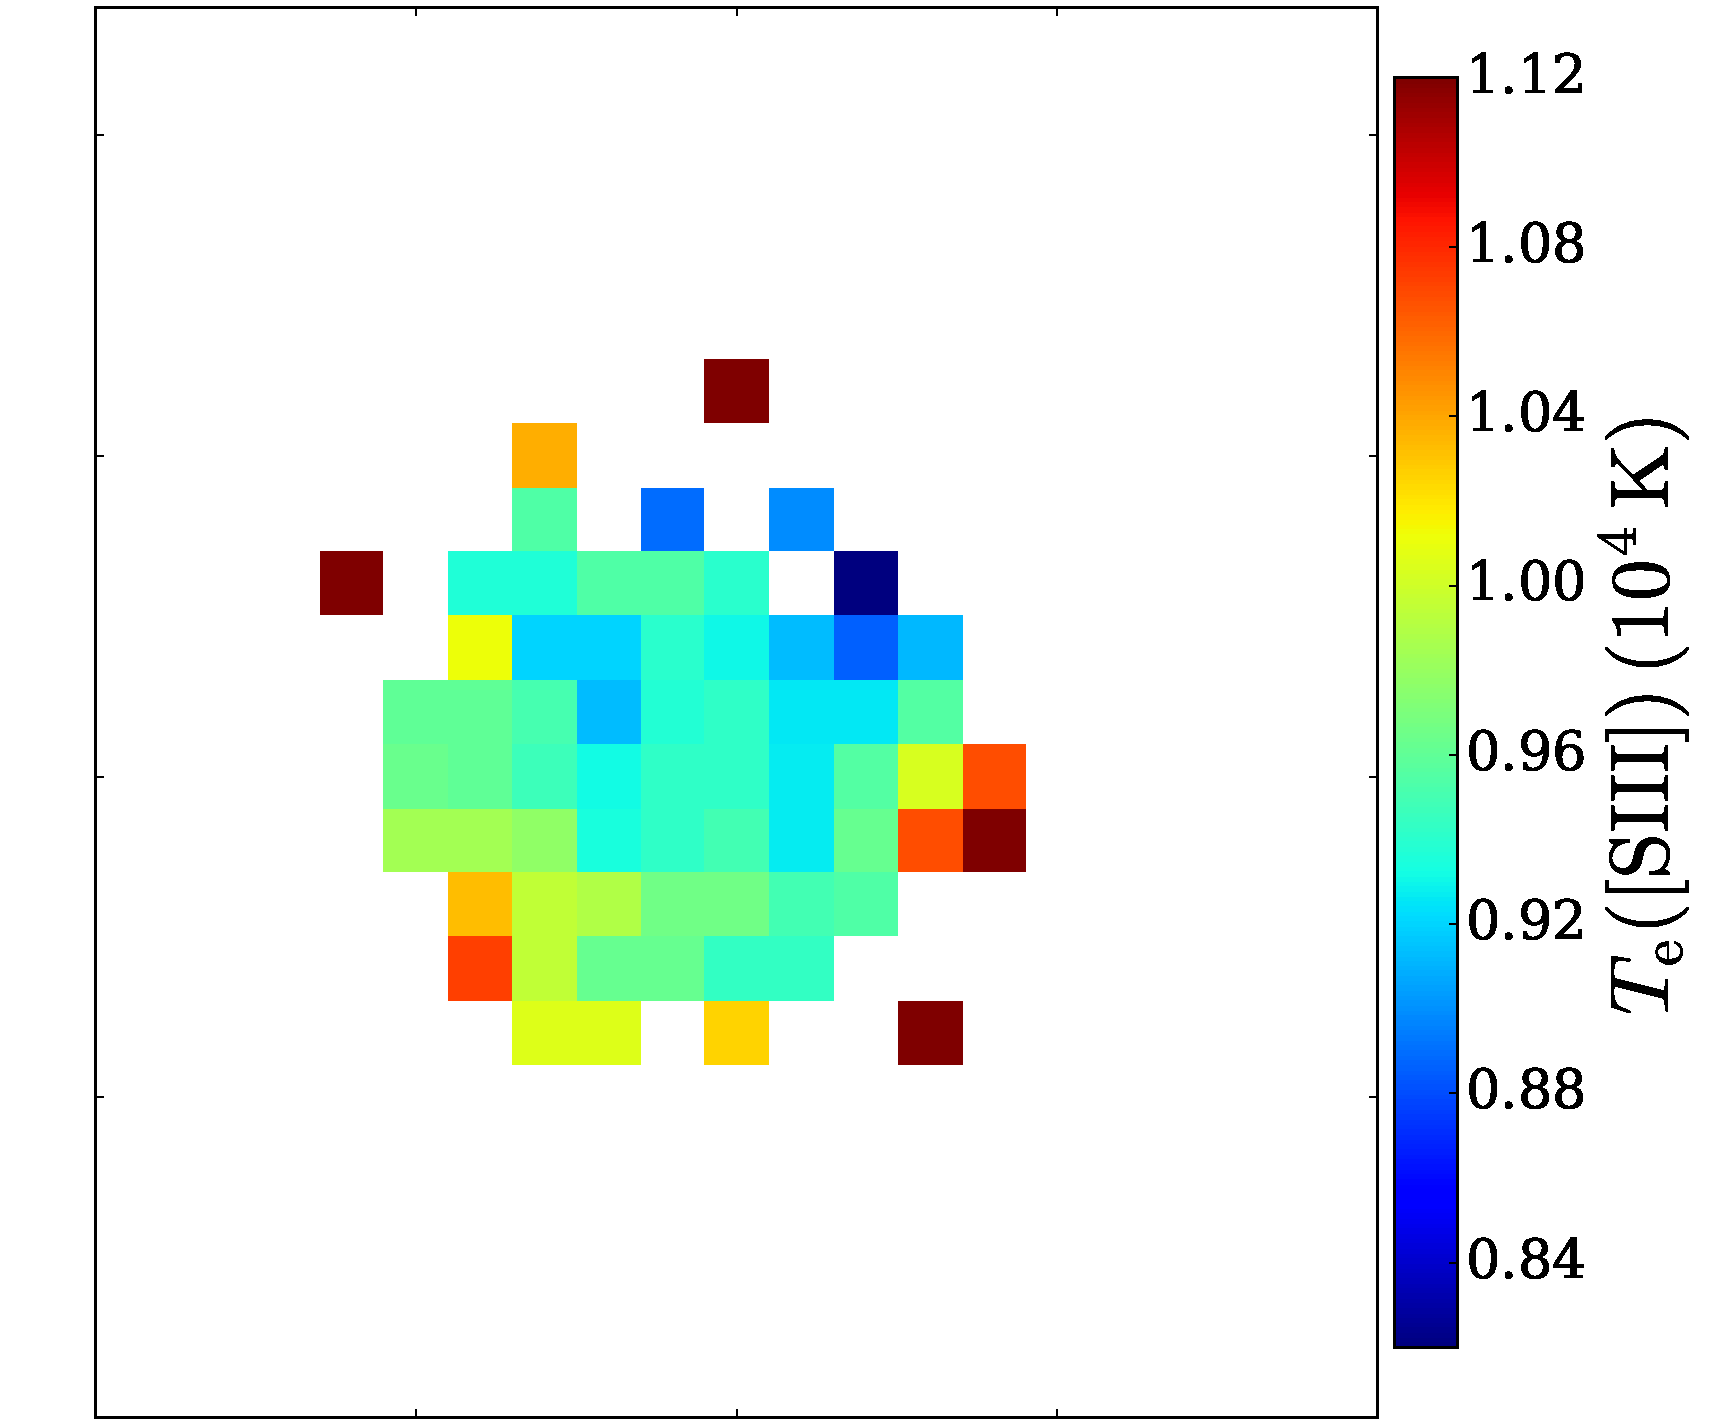
\includegraphics[width=0.999\linewidth]{Figs/MUSE_SN1998bw_T.pdf}
\end{subfigure}
\begin{subfigure}{.242\textwidth}
  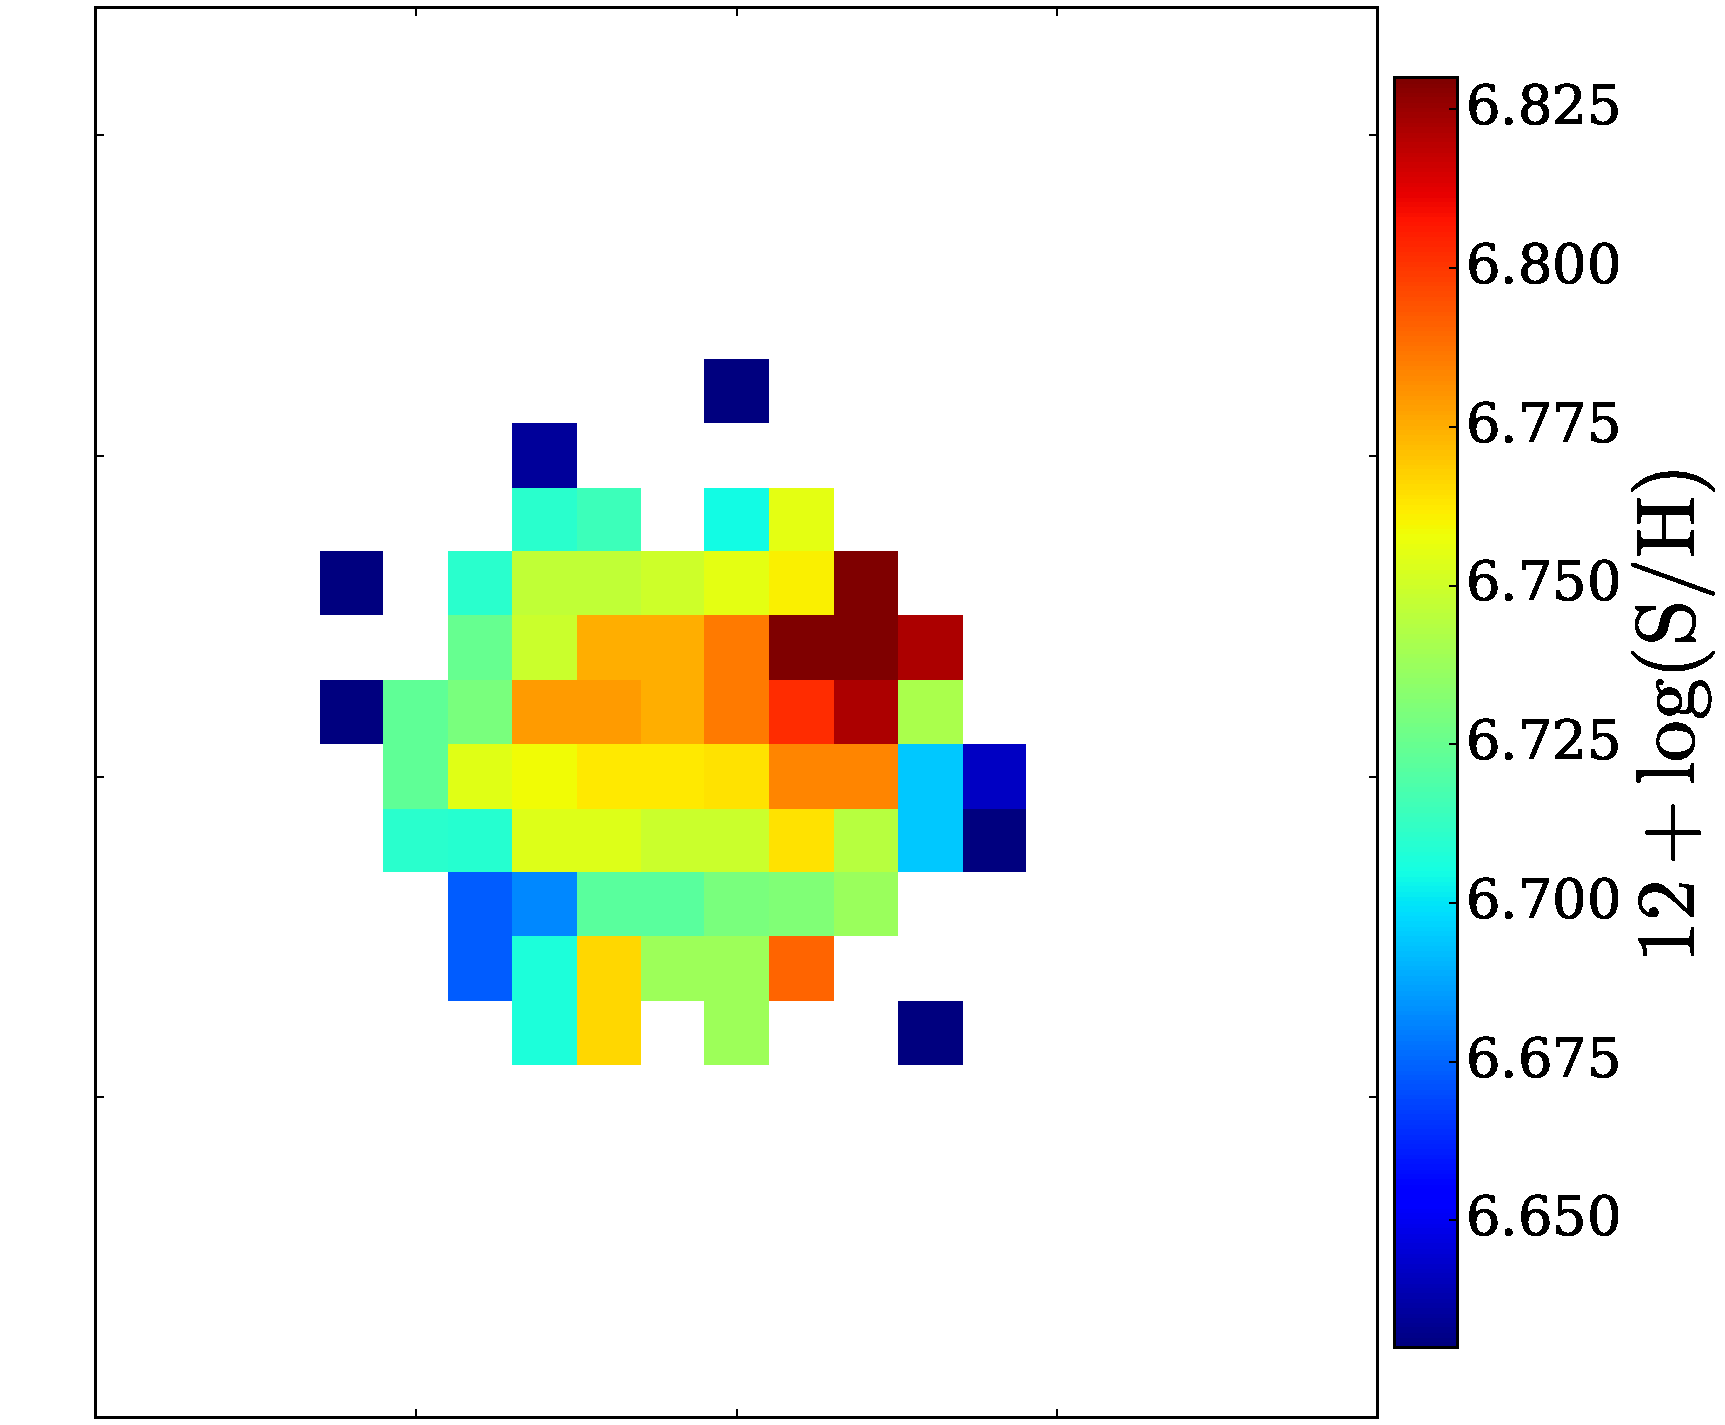
\includegraphics[width=0.999\linewidth]{Figs/MUSE_SN1998bw_SHTzoom.pdf}
\end{subfigure}
\caption{Zoom-in to the WR region for temperature estimation. top-left: nebular \siii($\lambda9069$), top-right: auroral \siii($\lambda6312$), bottom-left: \siii\, electron temperatures, bottom-right: $12+\log(\mathrm{S/H})$ as derived from the electron temperature. The solar abundance [O/S] is 1.57 \citep{2009ARA&A..47..481A}, so the $12+\log(\mathrm{S/H})$ scale corresponds to \oh = 8.2 to 8.4. All panels are approximately 6" by 6", or 1 by 1~kpc. One MUSE spaxel corresponds to 35~pc.}
\label{fig:temp}
\end{figure}

Given the strong constraints that these measurements of oxygen abundance could imply for the SN\,1998bw progenitor metallicity, we further seek to corroborate our earlier metallicities through those from temperature-sensitive lines. Unfortunately, the brightest of those auroral lines (\oiii($\lambda$4363)) is not covered by the MUSE wavelength response, and the other temperature-sensitive lines are too faint to be detected in most of the individual spaxels. However, we clearly detect both \siii($\lambda$6312) in the WR region (Figure~\ref{fig:temp}), and in integrated spectra around the SN position.



Following \citet{2013ApJS..207...21N}, we derive an electron temperature $T_{mathrm{e}}$ using \siii\, in the central part of the WR-region of around $T(\mathrm{e})_{\siii}=(0.94\pm0.04)\cdot10^{4}$~K. Figure~\ref{fig:temp} contains maps of the crucial emission lines (nebular \siii($\lambda9069$, and auroral \siii($\lambda$6312)), the resulting temperatures as well as sulfur abundances. These values correspond to somewhat larger temperatures of \oiii~of around $T(\mathrm{e})_{\oiii} \sim 1.07\cdot10^{4}$~K \citep{2006A&A...448..955I, 2012A&A...547A..29B}. The flux in the doublets of \oii($\lambda\lambda$7320,7330) and \oiii($\lambda\lambda$4959,5007) then yields central abundances of the WR region around \oh $\sim 8.3$.

Similar values are obtained when using solar abundances to convert the sulfur to an oxygen abundance. These are somewhat (0.1-0.2~dex.) higher than those implied by the strong line diagnostic from Sect. \ref{sec:mapoh}, but critically depend on the sulfur-to-oxygen temperature conversion or assumed abundance. They are thus subject to some systematic uncertainties. However, it is clear that the strong structure in O3N2 or N2 over the \hii-region are not observed in electron temperatures.

Emission-lines in the SN region are substantially fainter, and \siii($\lambda$6312) is only detected in a stacked spectrum extracted from 3x3 spaxels around the SN position yielding $T_{\mathrm{e}}(\siii)=(1.24\pm0.18)\cdot10^{4}$~K, slightly higher than in the WR-region, but with large uncertainties.

We also re-reduce archival VLT/FORS2 long-slit spectroscopy (Sect.~\ref{app:fors}) as it covers both WR-region and SN position and extends below $4000\,\AA$. Using the well-detected \oiii($\lambda$4363) line, we measure temperatures of $T_{\mathrm{e}}(\oiii)=(1.05\pm0.05)\cdot 10^{4}$~K and $T_{\mathrm{e}}(\oiii)=(1.29\pm0.18)\cdot10^{4}$~K for the WR and SN region, respectively, broadly consistent with the estimates from MUSE through \siii($\lambda$6312). They imply oxygen abundances of \oh=$8.36\pm0.07$ and $8.09\pm0.15$ for WR and SN region respectively.

Our relatively low oxygen abundances at the location of SN (\oh$\sim8.1-8.2$) and WR-region (\oh$\sim8.3-8.4$), as well as galaxy integrated values ($\sim8.2-8.3$) correspond to 0.2 to 0.4 times the solar value, and thus explain many of the long-wavelength properties of ESO184-G82 as typical for metal poor dwarf galaxies without invoking a deficiency in molecular gas \citep{2016arXiv160901742M}.


\subsection{Metallicity Gradients}
\label{sec:metgrad}

\begin{figure}
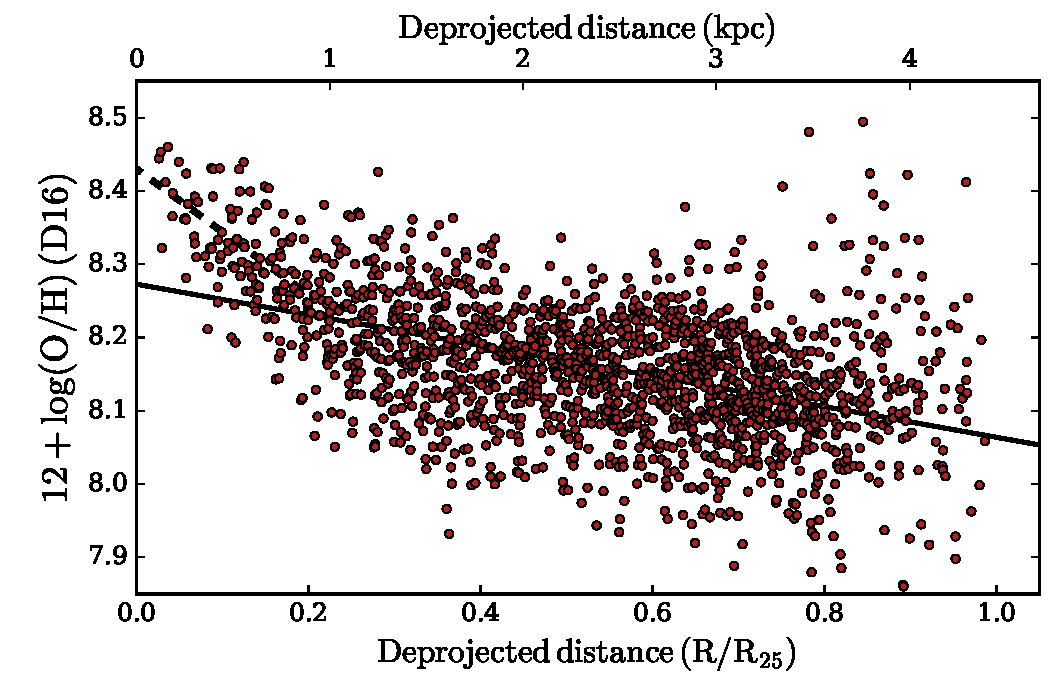
\includegraphics[angle=0, width=0.99\columnwidth]{Figs/MUSE_SN1998bw_metgrad.pdf}
\caption{Metallicity gradient for ESO184-G82. Each data point is a spaxel-based measurement of oxygen-abundance on the \citet{2016Ap&SS.361...61D} scale, where individual spaxels have been binned with their neighbors to enhance S/N if necessary.}
\label{fig:metgrad}
\end{figure}

The metallicity of galaxies is often observed to decrease with the distance from their centers \citep[e.g.][]{1994ApJ...420...87Z, 2014A&A...563A..49S}, also observed in the hosts of SNe \citep{2016A&A...591A..48G} or here (Figure~\ref{fig:s2}). These gradients are important to understand for spatially-unresolved studies at high redshift, where positional offsets can be measured, but abundances are only derived in a galaxy integrated manner. 

Using a linear regression on the data of Figure~\ref{fig:metgrad}, the metallicity gradient is best fit with a slope of $0.25\pm0.01$~dex/$R_{25}$ in relative, or 0.056~dex/kpc in physical scales, well in the range that was previously derived for galaxies of comparable stellar mass \citep{2015MNRAS.448.2030H}. Here, $R_{25}$ is the radius at the $B=25\,\mathrm{mag}\,\mathrm{arcsec}^2$ isophote. O3N2-based diagnostics return slightly steeper, but within errors generally compatible values. The linear fit to the oxygen abundance data is a reasonable description of the data, except for the very center (deprojected distance < 1~kpc), where the metallicity is seen to decrease more steeply. Limiting the fit range to this region, the slope in the central kpc is 0.18 dex/kpc (see dashed line in Figure~\ref{fig:metgrad}), but depends strongly on the metallicity diagnostic\footnote{A O3N2-based method returns a decreasing abundance towards the center, similar to what is seen also in a third of SN hosts in this diagnostic \citep{2016A&A...591A..48G}.}.

A comparison between this metallicity gradient to the typical values of (projected) GRB distances from the galaxy centers of 1.3~kpc \citep{2016ApJ...817..144B} does not provide strong reason to suggest that the average measurement of GRB host metallicities from spatially-unresolved data is significantly skewed when compared to the GRB site metallicity. There is however a non-negligible fraction of GRBs at substantial distances to their hosts (10\% at $>3$~kpc) where metallicity gradients might lead to overestimates on the GRB site abundance from unresolved spectra.

Figure~\ref{fig:metgrad} also illustrates the typical spread of oxygen abundances at a given galactic radius. With an root-mean-square (RMS) spread below 0.1~dex, and we find no evidence for extremely ($Z < 0.1 Z_\odot$) gas-poor regions at the spatial scales probed by our observation (100 pc). 

\subsection{ESO184-G82 if Seen at High Redshift}

GRB\,980425/SN\,1998bw is the closest GRB detected in two decades, and an exceptional opportunity to measure the physical parameters of its host within high precision and high spatial resolution. Typically, information on environments of GRBs or similar kind of transients  at higher redshift is obtained only through galaxy-integrated measurements \citep{2015A&A...581A.125K, 2016A&A...590A.129J}, where it is not necessarily obvious whether the measured parameters actually correspond to GRB/SN location properties. We thus compare the GRB explosion site spectrum extracted from the 9 closest spaxels to a galaxy-integrated spectrum as it would appear if it were unresolved and observed through a long-slit. 

First, we compare the total SFR as derived from integrating all spaxels after a reddening correction ($SFR=0.23\pm0.02$\,\Msunyr), to the value what would inferred from the \ha\,flux corrected from the $E_{B-V}=0.07\pm0.01$ derived from the integrated spectrum ($SFR=0.18\pm0.02$\,\Msunyr). Both values nicely agree with far-infrared, \oi, and \cii\, derived SFRs \citep{2014A&A...562A..70M, 2016arXiv160901742M}, and the narrow-band \ha\, image from \citet{2005NewA...11..103S} once their Salpeter IMF is taken into account. The difference to other \ha\,-derived SFR \citep{2006A&A...454..103H, 2008A&A...490...45C} is entirely due to an overestimated dust correction and a different IMF.

We then derive physical parameters from the spectra of the explosion site, the central part of the Wolf-Rayet region, and the integrated galaxy within a diameter of 50" around its center as summarized in Table~\ref{tab:prop}. Generally, there is decent agreement between many of the physical properties of the galaxy and the SN site spectrum. Not unexpectedly, resolved measurement of EWs at the SN site are somewhat higher, whereas both dust (by 0.02~mag) and oxygen abundance (by 0.1~dex) are somewhat lower at the SN site than for a galaxy integrated spectrum. However, ESO184-G82 thus does not provide strong evidence that GRB position spectra are markedly different from galaxy-integrated values. Whether this observation remains valid for a larger sample of GRB hosts remains to be seen, of course.

Comparing Table~\ref{tab:prop} with Figures~\ref{fig:s2}~and ~\ref{fig:metgrad} also illustrates that the oxygen abundance derived from a galaxy-integrated spectrum is not the central abundance of the galaxy \citep[see also e.g.,][]{2016A&A...591A..48G}. As the metallicity determination in an unresolved case is a SFR-weighted measurement, it is dominated by \hii-regions that are primarily located somewhat offset from the center as illustrated in Figure~\ref{fig:EW}. It thus corresponds to a measurement at a distance of around $2-3$ kpc from the center. 

\begin{table*}[!ht]
\caption{GRB~980425/SN~1998bw properties from extracted spectra\label{tab:prop}}
\centering
\begin{tabular}{cccc}
\hline
\hline\noalign{\smallskip}
 & {ESO184-G82} & {SN region} & {WR region} \\
\hline\noalign{\smallskip}

EW(\ha) (\AA)       & $56.0\pm1.4$ & $82\pm2$  & $>900$ \\
EW(\oiii)  (\AA)    & $34.5\pm0.9$ & $50\pm2$  & $>850$ \\
$E_{B-V}$ (mag)    & $0.07\pm0.01$ & $0.05\pm0.02$ & $0.21\pm0.01$ \\
$n_{e}$ (cm$^{-3}$) & $80\pm10$ & $90\pm10$ & $140\pm10$  \\
$T_\mathrm{e}$(\siii) ($10^4$~K)$^{\mathrm{(a)}}$ & $\cdots$ & $1.24\pm 0.18$ & $0.93\pm 0.01$\\
$T_\mathrm{e}$(\oiii) ($10^4$~K)$^{\mathrm{(a)}}$ & $\cdots$ & $1.29\pm 0.18$ & $1.05\pm 0.05$\\
\oh\, (D16)$^{\mathrm{(a)}}$ & $8.15 \pm 0.01$ & $8.06 \pm 0.01$ & $8.21 \pm 0.01$ \\
\oh\, (PP04, O3N2)$^{\mathrm{(a)}}$ & $8.32 \pm 0.01$ & $8.31 \pm0.01$ & $8.11 \pm 0.01$ \\
\oh\, (PP04, N2)$^{\mathrm{(a)}}$ & $8.34 \pm 0.01$ & $8.32 \pm0.01$ & $8.19 \pm 0.01$ \\
\oh\, ($T_\mathrm{e}$) & $\cdots$ &  $8.09\pm0.15$ & $8.37\pm0.07$ \\
SFR (\Msunyr) & $0.23\pm0.02$ & $\cdots$ & $\cdots$ \\

\hline\noalign{\smallskip}
\end{tabular}

\tablefoot{
\tablefoottext{a}{The quoted error is statistical only. There is an additional systematic error in each of these measurements due to various reasons. For the respective parameters, it is approximately $T_\mathrm{e}=0.1\cdot10^4$\,K, \oh\, (PP04, O3N2)=0.14~dex, \oh\, (PP04, N2)=0.18~dex. The systematic error on \oh\, (D16) is presently not well quantified, but we expect it in the range of $\sim$0.1~dex.}
} 
\end{table*}


\section{Conclusions and Summary}

SN1998bw represented the first solid observational evidence that linked GRBs with core-collapse supernovae, and since then has become the prototypical GRB/SN in terms of luminosity as well as spectral and temporal evolution. This very first GRB/SN has already demonstrated the absence of hydrogen and helium as well as broad absorption lines characteristic of a photosphere expanding at high velocities that should become typical of SNe following long GRBs in the later years.

In this article, we use new spatially-resolved spectroscopy obtained with the state-of-the art IFU MUSE over 10x10 kpc with individual spaxels covering 35 x 35 pc (effective spatial resolution of $\sim$100 pc) to study the properties of the hot gas phase and the stellar population at the SN position. We show that GRB~980425/SN1998bw exploded in a young (5 - 8 Myr old), dust-poor ($E_{B-V} = 0.03_{-0.03}^{+0.06}\,\mathrm{mag}$) environment. The ages of the stellar population correspond to life times of stars with ZAMS masses between approximately 25 to 40~M$_{\odot}$. A similar progenitor mass was derived from modeling the SN\,1998bw's nebular spectra \citep{2006ApJ...640..854M}, and provides evidence that the GRB formed in situ.

We derive a total SFR of $SFR=0.23\pm0.02$\,\Msunyr, and a metallicity gradient of $-0.06\,\mathrm{dex\,kpc^{-1}}$ for ESO184-G82, demonstrating that the typical offsets of at most few kpc for higher-redshift GRBs have a small impact on the abundance determination for GRB hosts on average. Also, emission-line-based parameters derived from the complete galaxy spectrum are dominated by the most star-forming regions and are thus a fair representation for the dust content and metallicity at the actual GRB explosion site.

Despite the uncertainty in the specific metallicity diagnostic, we can reach the following robust conclusions here with respect to abundances: Empirical strong-line methods based on \oiii/\hb\,and/or \nii/\ha\, fail to produce accurate maps of metallicity at the level of detail probed by our MUSE observation. They under/overpredict \oh\,in regions of high/low ionization parameter, respectively and therefore return an unphysical radial gradient in individual \hii-regions such that their centers appear to have lower metallicity. A recent method based on photoionization models and \sii\,from \citet{2016Ap&SS.361...61D} does not show this dependence on ionization and returns values that are broadly similar but somewhat lower (by up to 0.2~dex) than those from electron temperatures via the observed ratios of auroral-to-nebular \siii\,or \oiii. Taking these analysis into account, we consider \oh$\sim8.1$ at the SN position, \oh$\sim8.3$ for a galaxy integrated spectrum and \oh$\sim8.3$ for the nearby WR region as our best estimates of the respective metallicities. The immediate environment of GRB~980425 is thus indicating a progenitor with $Z\sim0.25\,\mathrm{Z}_\odot$ and $M_{\rm{ZAMS}}$ between $\sim 25$ and $\sim40~\mathrm{M}_{\odot}$ for this GRB.

\begin{acknowledgements}

Its a pleasure to thank D.~Malesani for providing broad-band imaging of the SN field and L.~Christensen for helpful discussion. T.K. and P.S. acknowledge support through the Sofja Kovalevskaja Award to P.S. from the Alexander von Humboldt Foundation of Germany. L.G. was supported in part by the US National Science Foundation under Grant AST-1311862. We acknowledge the use of \texttt{NumPy} and \texttt{SciPy} \citep{Walt:2011:NAS:1957373.1957466} for computing and \texttt{matplotlib} \citep{Hunter:2007} for creating all plots in this manuscript. 

\end{acknowledgements}


\bibliography{./bibtex/refs}

\begin{appendix}

\section{Re-analysis of Archival Long-slit Spectra}
\label{app:fors}

The ESO archive contains a number of high-quality, but low-resolution spectra obtained with the FOcal Reducer/low dispersion Spectrograph 2 (FORS2, \citealt{1998Msngr..94....1A}) that are particularly interesting in the context of this work. These are the same spectra used by \citet{2006A&A...454..103H}, and contain data taken with a 1\farc{0} slit on 2004-07-15 with the grism 600$B$ (3450\,\AA\, to 6050\,\AA\, with resolving power $R\sim850$) and on 2004-07-16 in grism 600$RI$ (5300\,\AA\, to 8450\AA\, with $R\sim1050$). The position angle during both observations was 28$^\circ$ from East such that both the SN and WR region are covered by the slit (Figure~\ref{fig:Host}). The total exposure time was 1350~s (each three individual frames with 300~s and 150~s) in the 600$B$ setup and 2250~s in the 600$RI$ (each five single frames with 300~s and 150~s) setup. We reduce and analyse this archival FORS2 data using standard procedures, specifically the ESO FORS2 pipeline in its version \texttt{5.3.8} and self-written methods and algorithms in python \citep{2015A&A...581A.125K}.

\begin{figure}
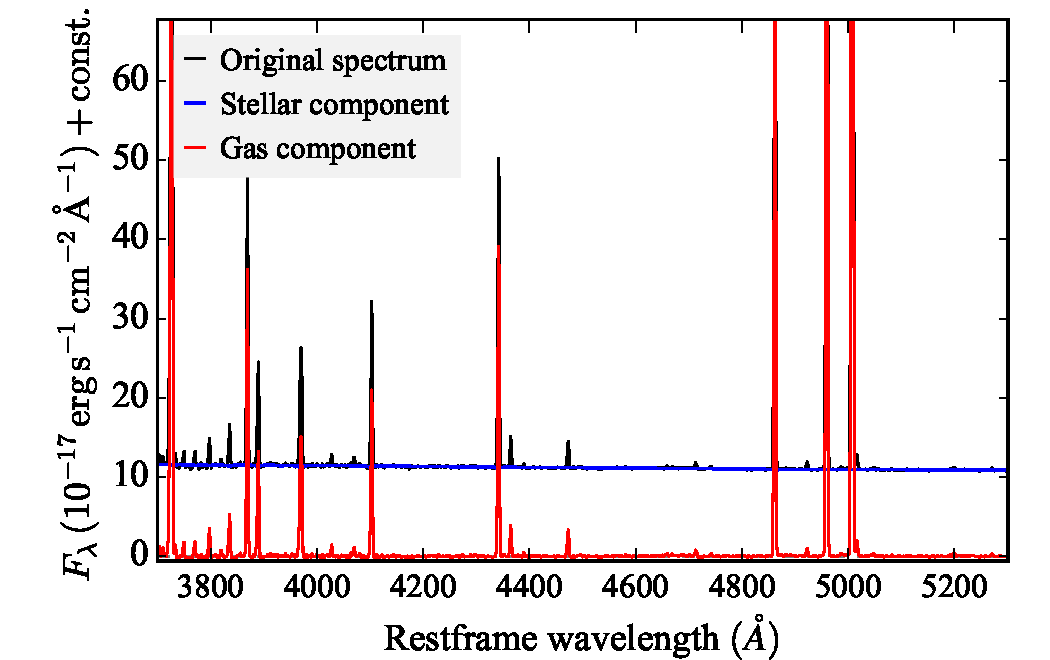
\includegraphics[angle=0, width=0.9\columnwidth]{Figs/FORS2_3700_5301_starlight.pdf}
\caption{FORS2 600$B$ spectrum of the brightest pixel of the WR region. Black is the original spectrum, blue the fitted stellar component, and red the resulting spectrum for the gas-phase only. Blue and black spectra are shifted to enhance clarity in the Figure.}
\label{fig:FORSWR}
\end{figure}

\begin{figure}
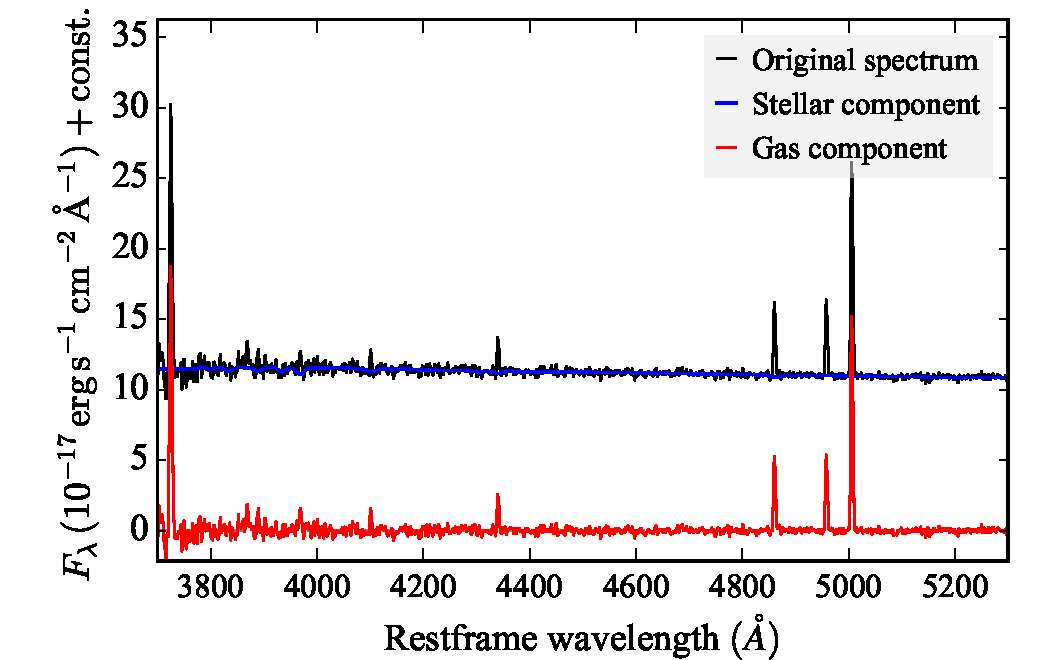
\includegraphics[angle=0, width=0.9\columnwidth]{Figs/FORS2_3700_5300_starlight.pdf}
\caption{FORS2 600$B$ spectrum of the explosion site. Black is the original spectrum, blue the fitted stellar component, and red the resulting spectrum for the gas-phase only. Blue and black spectra are shifted to enhance clarity in the Figure.}
\label{fig:FORSSN}
\end{figure}

In particular the 600$B$ (Figs.~\ref{fig:FFORSWR} and \ref{fig:FORSSN}) data are taken under excellent atmospheric conditions leading to a width of the spectral line spread function of FWHM=0\farc{6} at 5000\,\AA\, as evidenced by the trace of a stellar source serendipitously on the slit at a distance of 22\farc{0} to the WR region (also seen in Figure~\ref{fig:Host}). The 600$RI$ data have somewhat worse spatial resolution (FWHM=1\farc{0} at 7000\,\AA). This mismatch leads to the complication that the two different spectra are convolved with very different spatial scales. Due to the small angular size of the of WR region core ($\lesssim 0\farc{1}$ via HST imaging), and the gradient in physical properties, ratios of lines observed in the two different setups (e.g. for dust reddening distribution) are thus clearly non-trivial to interpret.

Table~\ref{tab:fluxes} contains line fluxes and equivalent widths from our analysis of the FORS2 spectra, sometimes significantly different to the \citet{2006A&A...454..103H} values. Their actual error on the line fluxes remains unfortunately unclear, but a substantial uncertainty by at least 25\% must be present (as estimated from the apparent discrepancy between their line-flux ratios of \oiii($\lambda$5007)/\oiii($\lambda$4959) and \nii($\lambda$6584)/\nii($\lambda$6548) to the theoretical value of 2.98 set by magnetic-dipole transition probabilities and observed in high-quality SDSS spectra \citep[e.g.][]{2000MNRAS.312..813S, 2006agna.book.....O, 2016MNRAS.459.3475W}.

\begin{table*}[!ht]
\caption{GRB~980425/SN~1998bw fluxes/EW from long-slit spectra\label{tab:fluxes}}
\centering
\begin{tabular}{ccccc}
\hline
\hline\noalign{\smallskip}
 &  \multicolumn{2}{c}{SN region$^{a}$} &  \multicolumn{2}{c}{WR region$^{b}$}  \\
 &  Flux$^{c}$ & EW$_{\mathrm{rest}}$ (\AA)  & Flux$^{c}$ & EW$_{\mathrm{rest}}$ (\AA) \\

\hline\noalign{\smallskip}

\oii($\lambda$3727)  & $47\pm2$ & $48\pm3$ & $41\pm3$ & $250\pm5$ \\
\neiii($\lambda$3968)& $4.3\pm0.6$ & $3.1\pm0.9$ & $8.2\pm0.2$ & $52\pm2$ \\
%\sii($\lambda$4072)  &  &  & $1.36\pm0.05$ & $10\pm1$ \\
H$\delta$            & $2.6\pm0.5$ & $3.6\pm0.8$ & $7.7\pm0.2$ & $51\pm2$ \\
H$\gamma$            & $5.6\pm0.5$ & $9.0\pm1.2$ & $14.7\pm0.3$ & $57\pm3$ \\
\oiii($\lambda$4363) & $0.6\pm0.2$ & $2.2\pm0.8$ & $1.54\pm0.05$ & $10\pm1$ \\
H$\beta$             & $12.4\pm1.1$ & $24\pm2$ & $34.6\pm1.4$ & $313\pm3$ \\
\oiii($\lambda$4959) & $12.9\pm1.2$ & $24\pm2$ & $68\pm2$ & $650\pm5$ \\
\oiii($\lambda$5007) & $40\pm2$ & $75\pm4$ & $205\pm4$ & $1980\pm20$ \\
\hline
\hline
\nii($\lambda$6548)$^{b}$  & $1.3\pm0.2$ & $5.0\pm1.0$ & $1.57\pm0.03$ & $25\pm1$ \\
H$\alpha$            & $38.5\pm1.6$ & $115\pm6$ & $77\pm2$ & $1220\pm20$ \\
\nii($\lambda$6584)  & $4.9 \pm 0.3$ & $15.9\pm1.8$ & $4.7\pm0.2$ & $79\pm3$ \\
\sii($\lambda$6717)  & $7.8 \pm 0.3$ & $29\pm2$ & $4.4\pm0.2$ & $87\pm3$ \\
\sii($\lambda$6731)  & $5.9 \pm 0.3$ & $20\pm2$ & $3.4\pm0.3$ & $70\pm3$ \\
\hline\noalign{\smallskip}
\end{tabular}

\tablefoot{
\tablefoottext{a}{To increase the S/N ratio, we include the adjacent two pixels in the extraction for the SN region.}
\tablefoottext{b}{Derived from the spectrum at the peak of the emission of the WR region.}
\tablefoottext{c}{Fluxes are given as $10^{-16}\,\mathrm{erg}\,\mathrm{s}^{1}\,\mathrm{cm}^{-2}$.}
\tablefoottext{d}{The double horizontal line separates the nebular lines that were taken in the two different FORS2 setups. Due to the different width of the line spread function and thus angular scales observed in both setups, the lines below and above the horizontal line cannot easily be used together to infer physical properties.}
} 
\end{table*}

From the \hb/\hg\, and \hb/\hd\, ratio, we derive an $E_{B-V}=0.22\pm0.03$~mag for the WR and $E_{B-V}=0.08_{-0.08}^{+0.23}$~mag for the SN region, both perfectly consistent with the MUSE data\footnote{We would measure significant dust reddening if we would not correct our \hb, \hg, or \hd\,fluxes for stellar Balmer absorption}. Also other properties are very similar to our IFU-based values as given in Table~\ref{tab:prop}.

Finally, we exploit the bluer response of the FORS2 600$B$ grism to derive an age of the \hii\,region through a fit using composite stellar templates in \texttt{starlight} in a similar manner as in the main text. The stellar population in the WR region is extremely young, and the \citet{2003MNRAS.344.1000B} template with an age of 1~Myr dominates the best fit by contributing $\sim$60-90\% to the total observed star light in various fits using different spectral templates and reddening laws. This very young age is consistent with the extremely high EW of \oiii\, and \ha\, (Table~\ref{tab:fluxes}), and the age constraints derived in the main text.

The SN region has prominent stellar components with ages of 5 Myr and 40 Myr (each contributing around 30\% to the best-fit composite template), the younger of which is again consistent with the age estimate from the \ha\,EW in the main text.

\section{Dependence of O3N2-derived Oxygen Abundance on Ionization Parameter}
\label{sec:abundancevsion}

\begin{figure}
\begin{subfigure}{.24\textwidth}
  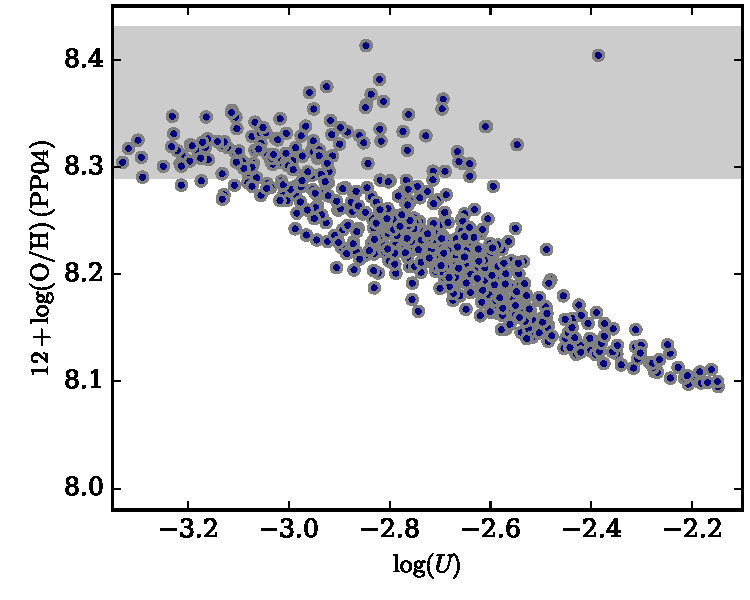
\includegraphics[width=0.999\linewidth]{Figs/QO3N2.pdf}
\end{subfigure}
\begin{subfigure}{.24\textwidth}
  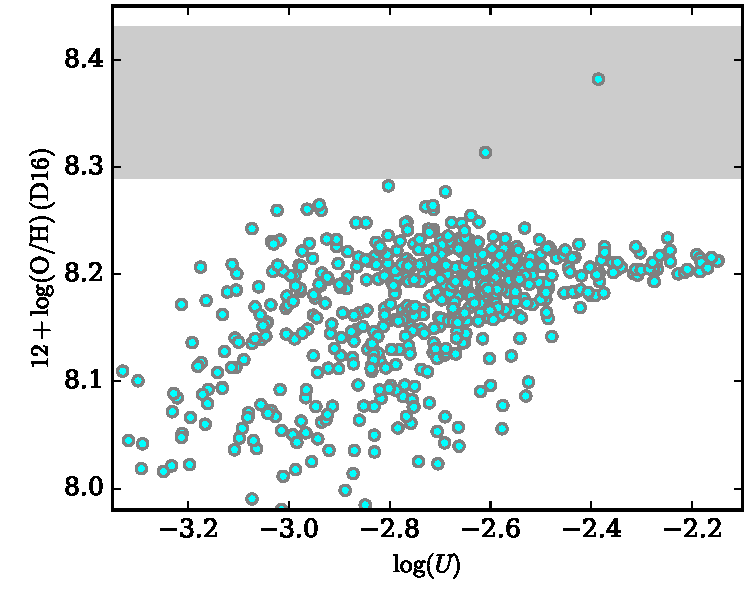
\includegraphics[width=0.999\linewidth]{Figs/QS2.pdf}
\end{subfigure}\caption{Dependence of the inferred oxygen abundance in two strong-line diagnostic ratios (left: O3N2 from \citealt{2004MNRAS.348L..59P}, right: S2 from \citealt{2016Ap&SS.361...61D}) on the ionization parameter $U$ (using the \siii\,to \sii\, ratio) for the WR region. Each data point corresponds to a single spaxel, and the grey region indicates the metallicity constraints from the temperature-sensitive \oiii($\lambda$4363) emission line.}
\label{fig:UO3}
\end{figure}

To better illustrate how a changing ionization parameter $U$ affects the metallicity measurement in the O3N2 or N2-scales we show $U$ (defined as ionizing photons per hydrogen atoms) versus \oh\, in the \citet{2004MNRAS.348L..59P} or \citet{2016Ap&SS.361...61D} scale of the brightest \hii-region in ESO184-G82 in Figure~\ref{fig:UO3}. Here, we use the \sii/\siii\,ratio (Figure~\ref{fig:s3s2}) to calculate $Q$ via photo-ionization models \citep{2011MNRAS.415.3616D}. Different parameterizations in $Q$ \citep[e.g.][]{2016A&A...594A..37M} do not change Figure~\ref{fig:UO3} significantly. The \sii/\siii\,ratio has the advantage of being nearly insensitive to metallicity, so we should not see a strong correlation between both quantities in accurate metallicity diagnostics. It is again clear, however, that the O3N2-based metallicity scale only reproduces the \hii-region metallicity in spaxels with low ionization parameter, and systematically under-predicts it at higher $U$. In contrast, the \citet{2016Ap&SS.361...61D} diagnostic is mostly independent on ionization parameter, but seems offset by an average $\sim$0.15~dex towards lower oxygen abundances (Figure~\ref{fig:UO3}, right panel).

\end{appendix}
\end{document}
